% +--------------------------------------------------------------------+
% | LaTeX Template                                                     |
% | for K-State Electronic Theses, Dissertations, and Reports          |
% |                                                                    |
% | Comments and guidelines for using the template are shown           |
% | within boxes like this one.                                        |
% |                                                                    |
% | Revised 6/30/06                                                    |
% | 9/14/06: Removed typos                                             |
% +--------------------------------------------------------------------+

% +--------------------------------------------------------------------+
% | Your paper should contain the following sections, except where     |
% | indicated as optional, in the order shown.  Also, all headings     |
% | shown with an asterisk (*) must be centered and in uppercase       |
% | letters:                                                           |
% |                                                                    |
% | Abstract Title Page (doctoral dissertations only)                  |
% | ABSTRACT* (doctoral dissertations only)                            |
% | Title Page                                                         |
% | Copyright Page (Optional - only needed if copyrighting)            |
% | ABSTRACT *                                                         |
% | TABLE OF CONTENTS *                                                |
% | LIST OF FIGURES *                                                  |
% | LIST OF TABLES*                                                    |
% | ACKNOWLEDGMENTS* (Optional)                                        |
% | DEDICATION * (Optional)                                            |
% | PREFACE * (Optional)                                               |
% | Individual Chapters                                                |
% | References and/or bibliography                                     |
% | Appendices (as needed)                                             |
% +--------------------------------------------------------------------+

% +--------------------------------------------------------------------+
% | The LaTex keyword \documentclass selects a particular class to     |
% | associate with the document.  The current documentclass            |
% | {class_diss} generates a Table of Contents that has leading dots   |
% | only on chapter subheadings.  If you prefer a Table of Contents    |
% | that has leading dots for all entries, replace {class_diss}        |
% | with {Mydiss} in the command below.                                |
% |                                                                    |
% +--------------------------------------------------------------------+

\documentclass[final, 12pt,oneside]{class_diss}

% +--------------------------------------------------------------------+
% | The following command sets the bibliography style to American
% | Institute of Physics (AIP).  Other styles are available in the
% | styles directory.  To use a different style, replace "aip" with
% | the filename of the style you want to use.
% +--------------------------------------------------------------------+

\bibliographystyle{unsrt}

\usepackage[utf8]{inputenc}
\usepackage[T1]{fontenc}
\usepackage[english]{babel}
% +--------------------------------------------------------------------+
% | Now, we add in all external packages that we will use throughout   |
% | the document.  You can add other packages as needed.
% +--------------------------------------------------------------------+

%\usepackage{     caption2} % Customize captions a bit more
\usepackage{      amsmath} % American Mathematics Society standards
%\usepackage{      wrapfig} % Wraps text around a figure or table
\usepackage{     graphicx} % Extended graphics package.
%\usepackage{     fancyhdr} % Efficiently handles headers and footers
%\usepackage{       braket} % Bra-Ket notation package
%\usepackage{     mathrsfs} % Specialized Math fonts (Hamiltonian, etc.)
%\usepackage{boxedminipage} % Boxed text can be produced
%\usepackage{     setspace} % Controls line spacing via \begin{space}

\usepackage{amsxtra}
\usepackage{amssymb}
\usepackage{amsthm}
\usepackage{latexsym}

% +--------------------------------------------------------------------+
% | The color package allows one to select colors for hyperlinking     |
% | (see below).                                                       |
% +--------------------------------------------------------------------+

\usepackage[usenames]{color}

% +--------------------------------------------------------------------+
% | Colors defined for use with this template.                         |
% +--------------------------------------------------------------------+

\definecolor{  Pink}{rgb}{1.0, 0.5, 0.5}
\definecolor{Maroon}{rgb}{0.8, 0.0, 0.0}

% +--------------------------------------------------------------------+
% | In the commands below, we use the 'natbib' package, and specify    |
% | the 'sort&compress' option, which condenses                        |
% | citations from (1,2,3,5,9,10,11) to (1-3,5,9-11).  The 'bibpunct'  |
% | option selects various parameters for how the citation will be     |
% | displayed.  In this case, only the comma (separation between       |
% | citations) and the 's' (superscript) arguments are chosen.  The    |
% | other curly braces deal with how to 'wrap' the citation (using     |
% | parentheses, brackets, etc.) and are not needed for the chosen     |
% | style.                                                             |
% +--------------------------------------------------------------------+

\usepackage[sort&compress]{natbib}
\bibpunct{}{}{,}{s}{}{}
\usepackage{hypernat}


% +--------------------------------------------------------------------+
% | Lastly, the hyperref package allows one to hyperlink cross-        |
% | references and figures in a LaTeX document.                        |
% +--------------------------------------------------------------------+

\usepackage[pdftex, plainpages=false, pdfpagelabels]{hyperref}

%tables
\usepackage{float}
\restylefloat{table}

\usepackage{enumitem}
\setlist[enumerate]{label*=\arabic*.}

\usepackage{multirow}


\hypersetup{
    linktocpage=true,
    colorlinks=true,
    bookmarks=true,
    citecolor=blue,
    urlcolor=red,
    linkcolor=Maroon,
    citebordercolor={1 0 0},
    urlbordercolor={1 0 0},
    linkbordercolor={.7 .8 .8},
    breaklinks=true,
    pdfpagelabels=true,
    }

% +--------------------------------------------------------------------+
% | Page margins are set on 1 inch on all sides.                       |
% +--------------------------------------------------------------------+

\topmargin      = -0.56in
\textheight     =  8.60in
\textwidth      =  6.46in
\oddsidemargin  =  0.02in

\setlength{\parskip}{1em}
% +--------------------------------------------------------------------+
% | The document finally begins here.                                  |
% +--------------------------------------------------------------------+
\begin{document}


  \setcounter{page}{-1}


% +--------------------------------------------------------------------+
% | Title Page -- Required for both Doctoral and Masters Students
% +--------------------------------------------------------------------+

% +--------------------------------------------------------------------+
% | Title Page
% +--------------------------------------------------------------------+
\newpage

% +--------------------------------------------------------------------+
% | This page should not contain a page number.  We use the
% | \thispagestyle[empty] command below to suppress page numbers
% | and other style elements.
% +--------------------------------------------------------------------+

\thispagestyle{empty}

% +--------------------------------------------------------------------+
% | The Title page begins here.
% +--------------------------------------------------------------------+

\begin{center}

   \vspace{1cm}

% +--------------------------------------------------------------------+
% | On the line below, replace "ENTER YOUR TITLE" with the title of
% | your ETDR.  Use all CAPITAL LETTERS.
% +--------------------------------------------------------------------+

   {\Large Edge provisioning for IoT}\\

   \vspace{0.5cm}



   \vspace{0.5cm}



   {\large Sergio A. Semedi Barranco}\\

   \vspace{0.5cm}




   MÁSTER EN INTERNET DE LAS COSAS. FACULTAD DE INFORMÁTICA\\
   UNIVERSIDAD COMPLUTENSE DE MADRID \\


   \vspace{0.65cm}
   \rule{2in}{0.5pt}\\
   \vspace{0.85cm}

  
\includegraphics[height=2.5in]{figures/escudo.jpg}
  

%+-- Escribe el nombre de tu asignatura de fin de master (Ingeniería de computadores,....)
   \vspace{0.5cm}
Trabajo Fin Máster en  Internet de las Cosas

   \vspace{0.5cm}





% +--------------------------------------------------------------------+
%  Fecha 
% +--------------------------------------------------------------------+

  ?-?-2020\\
   \vspace{1cm}

\end{center}

{\raggedleft
Director/es y/o colaborador:\\
   \vspace{ 1cm}
Francisco D. Igual Peña\\
Luis Piñuel Moreno\\
}


% +--------------------------------------------------------------------+
% | Use the section below if you have co-major professors.
% +--------------------------------------------------------------------+

%\begin{flushleft}
%   \hspace{10cm}Approved by:\\
%   \vspace{ 1cm}
%   \hspace{10cm}Co-Major Professor\\
%   \hspace{10cm}Enter Your Co-Major Professor's Name\\
%   \vspace{.5cm}
%   \hspace{10cm}Co-Major Professor\\
%   \hspace{10cm}Enter Your Co-Major Professor's Name\\
%\end{flushleft}

   \pdfbookmark[0]{Portada}{PDFPortadaPage}

% +--------------------------------------------------------------------+
% | Autorizacion Page -- Required for both Doctoral and Masters Students
% +--------------------------------------------------------------------+

% +--------------------------------------------------------------------+
% | Copyright Page
% +--------------------------------------------------------------------+

\newpage

\thispagestyle{empty}

\begin{center}

{\bf \Huge Autorización de difusión}

\vspace{1cm}

% +--------------------------------------------------------------------+
% | On the line below, replace "Enter Your Name" with your name
% | Use the same form of your name as it appears on your title page.
% | Use mixed case, for example, Lori Goetsch.
% +--------------------------------------------------------------------+

   \large Autor\\

   \vspace{0.5cm}

% +--------------------------------------------------------------------+
% | On the line below, replace Fecha
% |
% +--------------------------------------------------------------------+

   Fecha\\

   \vspace{0.5cm}
   \end{center}
   
El/la abajo firmante, matriculado/a en el Máster en Investigación en Informática de la Facultad de Informática, autoriza a la Universidad Complutense de Madrid (UCM) a difundir y utilizar con fines académicos, no comerciales y mencionando expresamente a su autor el presente Trabajo Fin de Máster: “TÍTULO”, realizado durante el curso académico 20XX-20XX bajo la dirección de XXXX [y con la colaboración externa de dirección de YYYY] en el Departamento de XXXX, y a la Biblioteca de la UCM a depositarlo en el Archivo Institucional E-Prints Complutense con el objeto de incrementar la difusión, uso e impacto del trabajo en Internet y garantizar su preservación y acceso a largo plazo.


   \pdfbookmark[0]{Autorización}{PDFAutorizacionPage}


   
   % +--------------------------------------------------------------------+
% | Copyright Page
% +--------------------------------------------------------------------+

\newpage

\thispagestyle{empty}

\begin{center}

{\bf \Huge Resumen en castellano}

  \end{center}
\vspace{1cm}

En este presente trabajo se realiza la implementación de EPFIOT (Edge Provisioning For Internet of Things). Una \textit{appliance} desarrollada para contemplar casos de Infraestructura como servicio en el \textit{edge computing} y específicamente preparada para interactuar con dispositivos IoT usando aceleradores hardware para IA.

En un mundo gobernado por el \textit{cloud computing}, surgen dudas sobre si de verdad es necesario mandar todos los datos que recogen los dispositivos a internet afrontando la latencia que esto supone, Epfiot es un proyecto que intenta usando pocos recursos ofrecerte esa nube de infraestructura para procesar los datos de tus dispositivos en tu propia red local, facilitándote maquinas en el borde con aceleradores IA para que tus dispositivos realicen inferencia sobre los datos rápidamente.

La aplicación ofrece una interfaz \textit{graphql} para montar un ecosistema IoT de infraestructura en el borde usando la virtualización de Linux (kvm) y otras tecnologías emergentes como puede ser LwM2M facilitando la configuración de los dispositivos.

\vspace{1cm}

% +--------------------------------------------------------------------+
% | On the line below, repla	ce Fecha
% |
% +--------------------------------------------------------------------+

\begin{center}

{\bf \Large Palabras clave}

   \end{center}

   \vspace{0.5cm}
   
   Internet de las cosas, Virtualización, Infraestructura como servicio, Computación en el borde, Nube, LWM2M, Red local, Aplicación, Enrutador, Maquina virtual
   



   
   \pdfbookmark[0]{Resumen}{PDFResumenPage}

    % +--------------------------------------------------------------------+
% | Copyright Page
% +--------------------------------------------------------------------+

\newpage

\thispagestyle{empty}

\begin{center}

{\bf \Huge Abstract}

  \end{center}
\vspace{1cm}

This work consist on the implementation of EPFIOT (Edge Provisioning For Internet of Things). An appliance developed to look at Infrastructure as a service based on the edge. It is specifically prepared for interacting with IoT devices using special hardware accelerators designed for AI.

Cloud computing is the only choice nowadays, certain doubts arise about if it would be mandatory to keep all device data sended directly to cloud assuming the latency costs. Epfiot relies in using low specs hardware trying to bring to your local area network a similar cloud model, simplifying the way of providing virtual machines through the use of real hardware accelerators for your devices. This will allow the device to perform inference over the collected data quickly.

The application has a graphql interface building an entire IoT ecosystem, using infrastructure on the edge thanks to Linux virtualization (kvm) and emerging technologies, like for example LwM2M to provide device bootstrapping.

\vspace{1cm}

% +--------------------------------------------------------------------+
% | On the line below, replace Fecha
% |
% +--------------------------------------------------------------------+

\begin{center}

{\bf \Large Keywords}

   \end{center}

   \vspace{0.5cm}
   
Internet of things, Virtualization, Infrastructure as a Service, IaaS, Edge computing, cloud computing, LWM2M, LAN, local area network, appliance, router, Virtual Machine
   



       \pdfbookmark[0]{Abstract}{PDFAbstractPage}
    \vfill


% +--------------------------------------------------------------------+
% | We use the following code to suppress page numbers and other
% | style issues we do not want present on a given page.               |
% +--------------------------------------------------------------------+

%\thispagestyle{empty} Looks like it's ok to remove this line
\newpage
\pagenumbering{roman}
\setcounter{page}{1}
\phantomsection
\addcontentsline{toc}{chapter}{Index}
\tableofcontents

%\listoffigures
%\listoftables

%\hfill  Are these lines necessary?
%\hfill

% +--------------------------------------------------------------------+
% | Acknowledgements Page
% |
% | If you choose not to have an Acknowledgements page, comment out
% | or delete the following 3 lines.
% +--------------------------------------------------------------------+

%% +--------------------------------------------------------------------+
% | Acknowledgements Page (Optional)                                   |
% +--------------------------------------------------------------------+

\newpage
\begin{center}
{\bf \Huge Agradecimientos}
\end{center}
\vspace{1cm}
\setlength{\baselineskip}{0.8cm}

%\pdfbookmark[0]{Acknowledgements}{PDF_Acknowledgements}

% +--------------------------------------------------------------------+
% | Enter text for your acknowledgements in the space below this box.  |
% |                                                                    |
% +--------------------------------------------------------------------+

Agradecimientos.....

%\phantomsection
%\addcontentsline{toc}{chapter}{Agradecimientos}

% +--------------------------------------------------------------------+
% | Dedication Page
% |
% | If you choose not to have a Dedication page, comment out
% | or delete the following 3 lines.
% +--------------------------------------------------------------------+

%% +--------------------------------------------------------------------+
% | Dedication Page (Optional)
% +--------------------------------------------------------------------+

\newpage
\begin{center}
{\bf \Huge Dedicatoria}
\end{center}
\vspace{1cm}
\setlength{\baselineskip}{0.8cm}

%\pdfbookmark[0]{Dedication}{PDF_Dedication}

% +--------------------------------------------------------------------+
% | Enter the text for your dedication in the space below this box.
% +----------------
Texto...
%\phantomsection
%\addcontentsline{toc}{chapter}{Dedicatoria}

% +--------------------------------------------------------------------+
% | Preface Page
% +--------------------------------------------------------------------+

%% +--------------------------------------------------------------------+
% | Preface (Optional)
% +--------------------------------------------------------------------+

\newpage
\begin{center}
{\bf \Huge Preface}
\end{center}
\vspace{1cm}
\setlength{\baselineskip}{0.8cm}

%\pdfbookmark[0]{Preface}{PDF_Preface}

% +--------------------------------------------------------------------+
% | Enter text of your Preface in the space below this box.
% +--------------------------------------------------------------------+

This template uses a separate file for each section of your ETDR:
title page, abstract, preface, chapters, reference, etc.  This
makes it easier to organize and work with a lengthy document.  The
template is configured with page margins required by the Graduate
School and will automatically create a table of contents, lists of
tables and figures, and PDF bookmarks.

Although the template gives you a foundation for creating your
ETDR, you will need a working knowledge of LaTeX in order to
produce a final document.  You should be familiar with LaTeX
commands for formatting text, equations, tables, and other
elements you will need to include in your ETDR.

This template uses a separate file for each section of your ETDR:
title page, abstract, preface, chapters, reference, etc.  This
makes it easier to organize and work with a lengthy document.  The
template is configured with page margins required by the Graduate
School and will automatically create a table of contents, lists of
tables and figures, and PDF bookmarks.

Although the template gives you a foundation for creating your
ETDR, you will need a working knowledge of LaTeX in order to
produce a final document.  You should be familiar with LaTeX
commands for formatting text, equations, tables, and other
elements you will need to include in your ETDR.

This template uses a separate file for each section of your ETDR:
title page, abstract, preface, chapters, reference, etc.  This
makes it easier to organize and work with a lengthy document.  The
template is configured with page margins required by the Graduate
School and will automatically create a table of contents, lists of
tables and figures, and PDF bookmarks.

Although the template gives you a foundation for creating your
ETDR, you will need a working knowledge of LaTeX in order to
produce a final document.  You should be familiar with LaTeX
commands for formatting text, equations, tables, and other
elements you will need to include in your ETDR.

%\phantomsection
%\addcontentsline{toc}{chapter}{Preface}

% +--------------------------------------------------------------------+
% | We use arabic (1, 2, 3...) page numbering starting from page 1.    |
% | Note, however, that there are many pages where this is not the     |
% | desired behavior - such as the Title page, or abstract.  In these  |
% | cases, we can use \thispagestyle{empty} to suppress page numbers,  |
% | and other general style issues that we've defined globally.        |
% +--------------------------------------------------------------------+

\newpage
\pagenumbering{arabic}
\setcounter{page}{1}

% +--------------------------------------------------------------------+
% | Here is where we include individual sections of the thesis or
% | dissertation.                                                      |
% +--------------------------------------------------------------------+

% +--------------------------------------------------------------------+
% | Chapters
% +--------------------------------------------------------------------+

% +--------------------------------------------------------------------+
% | Sample Chapter
% |
% | This file provides examples of how to
% | - insert a figure with a caption
% | - construct a table with a caption
% | - create subsections within the chapter
% | - insert a reference to a Figure or Table
% | - make a citation
% +--------------------------------------------------------------------+

\cleardoublepage

% +--------------------------------------------------------------------+
% | Replace "Chapter Title" below with the title of your chapter.  LaTeX
% | will automatically number the chapters.
% +--------------------------------------------------------------------+

\chapter{Introduction}
%\label{ch:Introducción}
\label{makereference}


% +--------------------------------------------------------------------+
% | Replace \section headings below with the title of your
% | subsections.  LaTeX will automatically number the subsections 1.1,
% | 1.2, 1.3, etc.
% +--------------------------------------------------------------------+

\section{Motivation}
\label{makereference1.1}

{\em Cloud computing} has been a major word speaking about data compute in the last decade; as of today, cloud computing is used to store, clean, process and analyze virtually every chunk of information gathered from any source.
%
With the emergence of Internet of Things (IoT), cloud computing is still a hot topic and an integral part in the deployment of complete infrastructures, prividing easy and scalable access to applications, resources and services, and being fully managed by  cloud service providers~\cite{cloud_def}.

IoT devices provide large amount of data, and hence cloud processing is a natural solution to deal with them. 
%
The {\em Cloud of Things} (CoT) term comes here into play,  deploying connected defices directly to the cloud to perform complex operations with the generated data using with Artificial Intelligence. This is the perfect tool for creating smart tasks that harness the immense amount of information.
%
However, Cloud Computing faces several challenges to meet the most stringent performance requirements of many application services, specially in terms of latency and bandwidth~\cite{IEE:Morabito:2017}.

To address and solve those problems, Edge Computing is a new paradigm that aims at bringing data storage and computation closer to the data source in order to improve response times and save data bandwidth. Edge Computing consists on increasing the resources available on the network edge, adopting a platform that provides intermediate layers for storing, cleaning, analyzing and inferencing.
%
Regarding the layers located at the edge, it is obviously impossible to provide the same kind of datacenter capabilities that are currently available in Cloud Computing premises. Edge Computing implies limited computational capabilities, so one of the main problems to be solved is to get similar cloud platforms (at least in terms of capabilities, flexibility and deployment mechanisms) into an edge environment with certain compute power for processing data.

Specifically, an edge computing infrastructure is based on a set of local hardware resources, that we have also adopted in this work. Specifically, we base our development on a fairly common hardware infrastructure composed of two main elements, namely:

\begin{itemize}
  \item \textbf{A Single Board Computer (SBC) or a minicomputer/barebone} that exhibit relatively high computing capacities with a proper reducing cost, energy consumption and form factor to adapt it to the specific scenario in which they are usually deployed.
  \item \textbf{Specific-purpose USB accelerators (DSAs)}, that provide co-processing capabilities to the central aforementioned computer (e.g. an Edge TPU as a Machine-Learning coprocessor). It accelerates specific tasks (e.g. inference processes for artificial intelligence models in the case of the Edge TPU), and can be selected depending on the typical application types that will be deployed on the edge infrastructure.
\end{itemize}

While the hardware problem is covered with the aforementioned elements, 
there are other elements involving the current paradigm of Cloud and Edge computing that are critical in order to develop an efficient and flexible edge architecture. 

\textbf{Virtualization} is the capability of creating virtual machines that act like real ones. This technology becomes mandatory in Cloud and Cdge Computing, since the creation of automatic elastic services requires getting rid of haphazard IT rooms, cables, and bulky hardware, reducing the overall IT overhead as well as management costs~\cite{virt_def}.

The creation and management of these virtual machines (VMs) would be impossible without the existence of \textbf{hypervisors}, pieces of software in charge of controlling the VM and providing a connection for the virtual resource and the real one.

\textbf{Virtual appliances} are VM images, usually with a specific configuration, designed to run on a virtual platform. They are designed to reduce or eliminate the installation, configuration, and maintenance costs associated with running suites of software~\cite{GEN:Virtualization:2010}.

When anything is able to connect to the Internet and generate data, there will be a possibility that at some stage uploading data to the cloud or sync device won't be necessary any longer. Temporarily, the data might not be required. In that scenario, either the device must be stopped from generating data or gateway device must decide when the data upload should be discontinued to avoid using network and cloud resources for a while.~\cite{Ficloud:AazaamHuh:2014}
Having this in mind and knowing that in a near future there are going to be millions devices called things connected, the \textbf{IoT gateway} appears to serve as a bridge for connecting these things, send data to the cloud or participate with an edge approach. A way to implement this edge gateway might be building a virtual appliance that will be situated close to the things. Figure ~\ref{figure1.1} shows a representation of the concept.


\newpage
\begin{figure}[h]%t=top, b=bottom, h=here
% \centering
    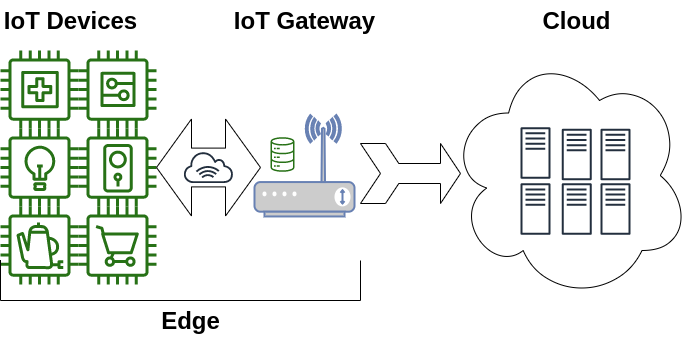
\includegraphics[width=6.5in]{figures/iot_gateway.png}
~\caption{Typical Gateway-based IoT deployment scheme.}
\label{figure1.1}
\end{figure}

Some of the features that could supply the IoT gateway are the following:

\begin{itemize}
  \item communication bridge
  \item data storage, filter and aggregation
  \item device management and configuration
  \item Security 
  \item route data
\end{itemize}

The presence of this Edge Layer facilitates the implementation of collaborative computing across devices, and it helps to apply data management policies. However, this edge layer is not usually rich in computing resources (mainly due to energy consumption limitations), which dramatically limits the approaches and designs that could be implemented to port move computing tasks to the edge. Following the Cloud-oriented approach of hypervisor-based virtualization, it can be proven that it can be cumbersome on these devices~\cite{arxiv:doluikiraly:2018}.
However we will see that this type of approach can be of great help using the proper hypervisor in order to gain the maximum efficiency.

\newpage
\section{Objectives}
\label{makereference1.2}

The main goal of the project is to prove that an IoT gateway using hypervisor-based virtualization reports improvements over an IoT edge environment is able to provide virtual machines capable of using real USB accelerators connected through a low spec motherboard.

Therefore with the purpose of show some results, a virtual appliance has been created running a custom service developed entirely from scratch using new technologies, these areas are highlighted in greater detail in the next chapters. 

With our appliance working, the next milestones are going to be evaluated:

\begin{itemize}
  \item Inference with virtual machines using real USB accelerators
  \item The feature of share real USB accelerators between multiple virtual machines
  \item Dynamic resource allocation including CPU or memory 
\end{itemize}

\subsection{Use case}
\label{makereference1.2.1}
Under the principles previously established it has been defined a use case that allows the appliance development to have a concise scenario in order to achieve better results. The project is aimed at apartments blocks, takes into account a modern building in which every house can be considered an smart house, having a large quantity of sensors across the area.

An external provider or a neighbourhood community wants to take advantage of EpFiot. That provider will be referred as client:
\begin{itemize}
  \item A low cost board will be deployed in base building of flats/apartments as an IoT Gateway with Epfiot appliance installed.
  \item Client will provide each apartment with sensors (temperature, humidity, camera, gas...).
  \item Epfiot appliance will have GPU accelerators physically connected through usb ports.
  \item Epfiot appliance will provide a service to the client allowing the spawn of customized vms that have direct access to the gpu accelerators.
  \item Client will be able to configure sensors using epfiot.
  \item Client will have full access and management for the vms and he will be able to allocate some resources including the usb accelerators.
  \item Sensors will generate data, instead of sending this data directly to internet, a proper vm could receive the data and use a accelerator for perform inference.
  \item Results could be stored in epfiot or another application in a low latency context.
\end{itemize}

Figure ~\ref{figure1.2} shows a representation of the case listed above.

\begin{figure}[h]%t=top, b=bottom, h=here
% \centering
    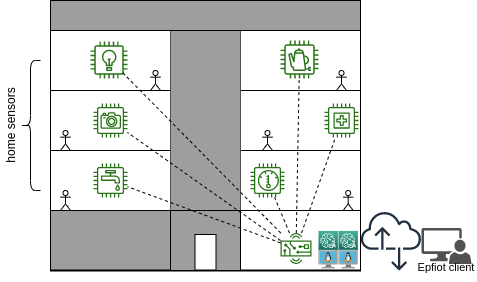
\includegraphics[width=6.5in]{figures/use_case.png}
~\caption{epfiot use case example}
\label{figure1.2}
\end{figure}

\newpage
\section{Document Organization}
\label{makereference1.3}

This document contains 7 chapters described as follow:

\begin{itemize}
  \item \textbf{Chapter 1, Introduction:} This chapter introduces a set of conceptual definition that is going to be mentioned along the document. This chapter also displays the complete project 's purpose through the explanation of its motivations and goals.
  \item \textbf{Chapter 2, State of the Arts:} This section displays the current state of Edge computing from a infrastructure point of view, discussing the underlyng technologies together with the advantages and disadvantages of each option. Finishing by a brief overview of related projects.
  \item \textbf{Chapter 3, Development Environment:} A list of the main technologies used for Epfiot will be enumerated, underlining what kind of utility is used for the project. Hardware and requirements are also discussed in this chapter.
  \item \textbf{Chapter 4: Architecture}: The chapter describes the overall architecture of Epfiot, reviewing every component and how they are connected between each other. 
  \item \textbf{Chapter 5: Features:} This part explains in detail the features of the project, end-user's functionalities are listed.   
  \item \textbf{Chapter 6: Results:} This section is about showing the final results that are obtained with the Epfiot application running. 
  \item \textbf{Chapter 7: Conclusions and Future Work:} Finally a brief summary of the project commenting what kind of implications it has and how to improve the current status of the project in a near future. 
\end{itemize}

%Here's an example of a citation to a single
%work.~\citet{CT:Weiner:1999} It's also possible to make multiple
%citations.~\citet{CT:Phillips:1985, ARP:Loy:1974}

% +--------------------------------------------------------------------+
% | Sample Chapter 2
% +--------------------------------------------------------------------+

\cleardoublepage

% +--------------------------------------------------------------------+
% | Replace "This is Chapter 2" below with the title of your chapter.
% | LaTeX will automatically number the chapters.
% +--------------------------------------------------------------------+

\chapter{This is Chapter 2}
\label{makereference2}

In this chapter, I want to refer to Chapter~\ref{makereference},
so I'm going to use the slash ref command along with the
"makereference" label which I assigned back at the beginning of
Chapter 1.

\section{Page Number References}
\label{makereference2.1} I should also be able to refer to a
specific page number, such as page~\pageref{makereference}.  Of
course, I'll need to have a slash label command and a unique name
in each section that I want to be able to refer to later in the
text.

\section{Referring to Sections Within Chapter 1}
\label{makereference2.2} Now, I'm going to refer to different
sections within Chapter 1. I gave an example of a figure in
section~\ref{makereference1.1} and an example of a table in
section~\ref{makereference1.2}.  In
section~\ref{makereference1.3}, we looked at examples of
bibliographic citations.

% +--------------------------------------------------------------------+
% | Sample Chapter 3
% +--------------------------------------------------------------------+

\cleardoublepage

% +--------------------------------------------------------------------+
% | Replace "This is Chapter 3" below with the title of your chapter.
% | LaTeX will automatically number the chapters.
% +--------------------------------------------------------------------+

\chapter{Development environment}
\label{makereference3}

This chapter explains the technologies and hardware components used in the project. Epfiot is delivered in the form of an appliance, what means that a proper virtual image  has been prepared specifically for the project, this 'custom' image will run software developed for Epfiot in particular (in fact, it has the same name) from scratch.

Details of this software are found in this Chapter because it's the most complex part, however there are many factors that are needed to take into account in order to get the complete overview for example, real host preparation, the appliance content itself and the already tuned image prepared directly for the client's use. Next sections contain a summary of the whole environment.

The project can be found in Github: \url{https://github.com/Semedi/epfiot} with a MIT license.


\section{Host}
\label{makereference3.1}

The Host is the physical machine that is going to contain the project so it is a very important part. Epfiot is situated in an edge context, what it means that the machine should cover some basics as described in chapter \ref{makereference1.1} and chapter \ref{makereference2.1}. However Epfiot has some minimum requirements that the host has to meet.

\newpage
\subsection{Minimum requirements}
\label{makereference3.1.1}

In the next list you can find a brief view of the hardware requirements:

\begin{itemize}
    \item Linux Support kernel > 2.6.2  0
    \item 64 bits architecture
    \item Intel Virtualization Technology (VT-x) or AMD's equivalent
    \item Intel Virtualization Technology for Directed I/O (VT-d) or AMD's equivalent
    \item Compatible usb accelerator
\end{itemize}

Those requirements should be accomplished in order to reach the desired virtualization for the project.
Intel Virtualization Technology ~\cite{vtx} enables a CPU to act as if you have several independent computers, in order to enable several operating systems to run at the same time on the same machine.

Usb Accelerator is going to be discussed in section \ref{makereference3.1.3}

\subsection{Software Requirements}
\label{makereference3.1.2}

The Epfiot appliance can run in every virtualization platform, however the provided projects driver can work with the following requierements:

\begin{itemize}
    \item KVM kernel module as hypervisor
    \item QEMU as hardware emulator
    \item Libvirt as a virtualization interface
    \item OpenSSH server, for custom operations requested by the appliance
\end{itemize}

\textbf{KVM} ~\cite{kvm} stands for Kernel-based Virtual Machine and is a full virtualization solution for Linux that can work with some virtualization extension as shown in ~\ref{makereference3.1} Intel Vtx, Vtd. It consist on a loadable kernel module that is the core virtualization infrastructure, bringing to the vms the possibility of interact with the host real hardware.

Basically kvm turns the Linux kernel into an hypervisor taking into advance some features like memory management or process scheduling. KVM have an userspace API and it is exposed via ioctls.
\textbf{QEMU} will use this userspace API. This software is the responsible of creating the hardware with a guest operating system running on the top. QEMU ~\cite{virtualization}interfaces with Linux, especially the KVM module within Linux, to directly run virtual machines on the physical hardware (and are not emulated by QEMU).

\textbf{Libvirt} is an open source API, daemon and a complex tool for managing this virtualization environment. ~\cite{libvirt}

Finally an OpenSSH server is needed to perform some basics IO operations between the host and the guest (Epfiot). The server should be configured only allow paswordless operations with a user capable of managing guest from kvm.

\subsection{Networking setup}
\label{makereference3.1.3}

There are several options in order to configure the host networking part, it is possible to create your own Linux bridge but it is advisable to use the networking mechanism that Libvirt virtualization API provides.
To define a Linux bridge we can refer to the term as Virtual switch, a kind of virtual device in your host server that the virtual machines use for 'plug in' and directs the networking traffic.

To achieve an environment with a minimum security associated, a Libvirt routed network is recommended.


\begin{figure}[h!]%t=top, b=bottom, h=here
\centering
    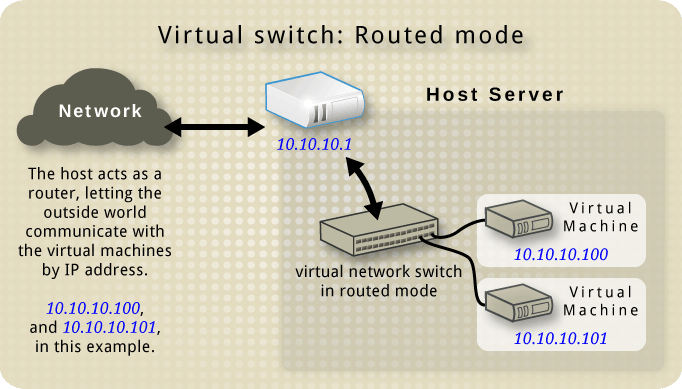
\includegraphics[width=4in]{figures/libvirt_routed_mode.png}
~\caption{Libvirt routed network. \cite{libvirt_networking}}
\label{figure3.1}
\end{figure}

With routed mode, the bridge is connected to the physical host LAN, passing guest network traffic back and forth without using NAT. This bridge sees the Ip in each packet and decides what to do. This mode gets all virtual machines in the subnet, routed through the bridge. The downside is that it is necessary to configure routers in order to get full access to the physical network. See Figure \ref{figure3.1}.

Also Epfiot takes benefit from Libvirt managed network because it has a DHCP feature that allows to generate virtual machine Ip addresses, making the effort of networking easy through dynamic network cards.

At this point, kernel parameters such as IP forwarding, and the proper NAT rules should be configured. Epfiot project comes with a set of networking script that makes this task easier.


\subsection{Tested Hardware}
\label{makereference3.1.3}
\subsubsection{Board}

In the execution of the project has been used the Intel NUC NUC5i5RYK with all the requirements below. It is a designed computer proposed by Intel which focuses on a high performance and small size.
Those characteristics fits perfectly with the Edge computing context, that is the reason to be selected as the board for this project.

Check the next table for more specifications of the device:

\begin{table}[H]
    \begin{center}
    \begin{tabular}[b]{|l|l|}
        \hline
        \textbf{NUC5i5RYB} & \\
        \hline
        Internal drive & M.2 SSD\\
        Processor & Intel® Core™ i5-5250U \\
        Cores	 & 2\\
        Threads & 4\\
        Base Frequency & 1.60 GHz\\
        Turbo Frequency & 2.70 GHz\\
        Memory size & 16 Gb\\
        Memory Type & DDR3L-1333/1600 1.35V SO-DIMM\\
        Memory Bandwitcth & 25.6 GB/s\\
        Memory Channels & 2\\
        Max DIMMS & 2\\
        Graphics &  Intel® HD Graphics 6000\\
        USB ports & 6\\
        Vtx & yes\\
        Vtd & yes\\
        \hline
    \end{tabular}
    \caption{Intel Nuc 5 specifications. ~\cite{nuc_specs}}
    \label{table1}
   \end{center}
\end{table}

\subsubsection{Usb accelerator}
As explained in this section \ref{makereference1.1}, Epfiot provides to the user the experience of using virtual machines connected to real usb accelerators, taking advance of the compute performance when realizing inference.

New Google coral was used in the project. Coral is a complete toolkit to build products with local AI. The on-board Edge TPU coprocessor is capable of performing 4 trillion operations per second (TOPS), using 0.5 watts for each TOPS.

Check the next table for more specifications of the device:

\begin{table}[H]
    \begin{center}
    \begin{tabular}[b]{|l|l|}
        \hline
        \textbf{Google Coral} & \\
        \hline
        ML accelerator & Google Edge TPU coprocessor\\
        Connector & USB 3.0 Type-C\\
        Dimensions & 65 mm x 30 mm\\
        \hline
    \end{tabular}
    \caption{Google coral specs ~\cite{coral_specs}}
    \label{table1}
   \end{center}
\end{table}


Notice that there are several Usb accelerators that could work with Epfiot solution similar to Google Coral, this device is used in this project with a test purpose.

\begin{figure}[h!]%t=top, b=bottom, h=here
\centering
    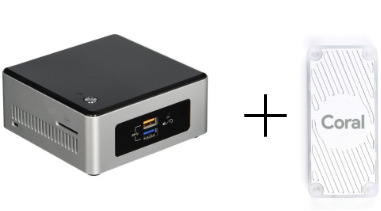
\includegraphics[width=4.5in]{figures/hardware.png}
~\caption{Devices used in Epfiot.}
\label{figure3.2}
\end{figure}
\newpage

\section{The Appliance}
\label{makereference3.2}
The most important part of the Epfiot project relies in the Appliance. A virtual machine has been prepared with for the sake of serve a custom application that has been designed, developed and implemented thinking in this edge computing particular scenario.

This appliance running Epfiot, will be responsible of managing virtual machines, altogether with the devices connected to the host (usb accelerators), providing a multi-tenant environment, storing a persistent model, bringing a secure interface to the user among other things.

You can find some more details regarding these technologies of the development process in the next sections. The architecture of the application will be discussed in the next chapter.

\subsection{Operating System}
\label{makereference3.2.1}
\textbf{Alpine Linux} is the selected appliance for the operating System. It is a security-oriented, lightweight Linux distribution based on musl libc and busybox.
The decision was made taking into account the small footprint that the image leaves after installing Alpine and the resulting low consumption. 

For holding the image the \textbf{qcow2} format was selected, stands for 'Copy on Write' a very common term in the computer science field and uses a disk storage optimization strategy that delays allocation of storage until it is actually needed. Basically the image will grow only if the mounted file system needs more space. This is the format used not only for the application, but also for all virtual machines that Epfiot would manage.

\begin{figure}[h!]%t=top, b=bottom, h=here
\centering
    
\includegraphics[width=3in]{figures/alpine.png}
~\caption{Alpine Linux logo}
\label{figure3.3}
\end{figure}
\newpage


\subsection{Epfiot Package}
\label{makereference3.2.2}

Once the host part is covered and a virtual machine created with the operating system selected, it is time to explain the most complex part of the project, the Epfiot software, a custom package that has been made exclusively for this thesis. 

A brief scheme of the Epfiot appliance in the overall architecture of the project covered in this chapter is shown in the Figure \ref{figure3.3}.

\begin{figure}[h!]%t=top, b=bottom, h=here
\centering
    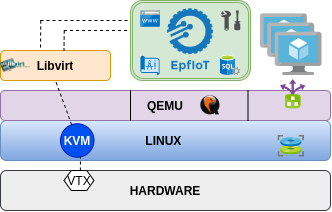
\includegraphics[width=5.5in]{figures/Epfiot_appliance.png}
~\caption{Epfiot appliance overview}
\label{figure3.3}
\end{figure}

The Epfiot package is a service that runs in the appliance that is composed by two major components:
\begin{itemize}
    \item Epfiot main application: \url{https://github.com/Semedi/epfiot}
    \item Epfiot Bootstrap Service: \url{https://github.com/Semedi/epfiot_bootstrap}
\end{itemize}

This subsection will explain the underlying technologies used in both components. On the other side, this will be used as an introduction for Chapter ~\ref{makereference4}. 
\newpage

\subsubsection{Epfiot Main application}

The Epfiot Main application is the heart of the project, its a piece of Software built from scratch that aims to fill all the purposes related in Chapter ~\ref{makereference1.3}. Before performing a deep dig into the architecture and the API interface of the project, main technologies will be arranged in order to grant a clear view to the reader.

\textbf{Dependencies}

\begin{enumerate}    
  \item alpine-sdk
  \item libvirt-dev
  \item libvirt-qemu
  \item cdrkit
  \item golang > 1.10.4
  \begin{enumerate}
    \item Epfiot
    \item libvirt-go
    \item net-http
    \item graphql-go
    \item gorm
    \item libvirt-go-xml
    \item ...
  \end{enumerate}

\end{enumerate}
The whole application has been developed using ~\textbf{git} as a version control system and hosted on Github. 
\textbf{Golang} was the selected language for this application. Go is an open source programming language that makes it easy to build simple, reliable, and efficient software.
Since Epfiot is a complex systems software and it is imperative that golang main purpose is to bring into the community an easy systems languaje, easy to learn, Golang was set as the best choice for developing Epfiot.

\begin{figure}[h!]%t=top, b=bottom, h=here
\centering
    
\includegraphics[width=3.0in]{figures/golang.png}
~\caption{Golang logo \cite{golang}}
\label{figure3.4}
\end{figure}

\newpage
Some of the advantages of using Golang that benefits Epfiot are:

\begin{itemize}
    \item Language Design: unlike other languages like C++, the designers of the language made a conscious decision to keep the language simple and easy to understand.
    \item Binaries: allowing the maintainer to administer a compiled version of the software. In this case the whole appliance is provided but it is possible to download the standalone epfiot distribution and install it in any x86 platform.
    \item Powerful standard library: As a system language this feature allow the developer to perform system calls and io operations in a safer way.
    \item Static Typing: Saving time debugging run-time errors.
    \item Concurrency Support: Ideal for a multi-tenant edge computing service.
    \item Package Management: Making easy to deal with dependencies.
\end{itemize}

Knowing the foundations stones of the project, it's time to show some key technologies:

\textbf{Libvirt, Qemu, KVM}: At this point these concepts should be very clear. The host operating system must have the Libvirt daemon running in the background (it is recommended to have the service enabled on systemd). In the appliance side, libvirt-qemu and libvirt-dev are needed. libvirt-qemu is a client of the libvirt daemon, by the other hand libvirt-dev contains the proper development headers. Libvirt-go which is a golang library is the binding for those headers, allowing the developer to build libvirt-tools using golang.

Libvirt uses xml for template definitions, which means that every resource created with libvirt must exist in a xml form. Managing templates with XML is a tedious thing, that's why libvirt-go-xml is brought into scope. This library handles the complex xml operations for building the document leaving behind a much simpler interface. Epfiot uses this library for building the templates. Those templates are sent to the host daemon using the libvirt client. Finally the libvirt daemon in the host side, knows how to instantiate the templates emulating the hardware on QEMU and granting kvm hypervisor capabilities for managing the guest.

\begin{figure}[h!]%t=top, b=bottom, h=here
\centering
    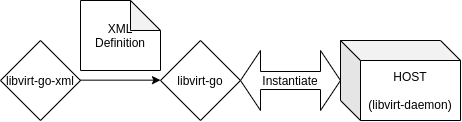
\includegraphics[width=3.9in]{figures/libvirt-xml.png}
~\caption{Libvirt basic scheme}
\label{figure3.4}
\end{figure}

\newpage

Libvirt ~\cite{libvirt_rpc} includes a basic protocol and code to implement an extensible, secure client/server RPC service. That is why Epfiot is able to communicate with the host in order to perform vm operations.
Trying to get a secure environment, Epfiot uses this rpc protocol tunneled over ~\textbf{SSH}. Epfiot takes profit of this situation using ssh for other mandatory tasks such as file system operations on the host machine.

Virtualization basics has been covered, let's move to net-http part.
\textbf{Net-http and graphql-go} correspond to Epfiot's service module. This module will be covered in detail all together with the others components in the next chapter, however, the technologies regarding this module will be explained below.

Golang languaje provides a good library for making http servers. Epfiot uses this library in order to build an interface to the end-user. At the time of building this interface, the most common design is usually famous REST API, nevertheless, a new technology was discovered replacing REST.
\textbf{GraphQL} ~\cite{graphqh_paper} is a framework with a query languaje that is used to express the data retrieval request issued to Web servers. This query languaje will behave taking into acount an schema that the developer should define.

Graphql gives clients the power to ask for exactly what they need and nothing more, makes it easier to evolve APIs over time, and enables powerful developer tools. These characteristic makes graphql very suitable for IoT, building this kind of service will save a lot of time since it does not require the design of new endpoints for every operation that the creator wants to expose.

Graphql-go is a graphql implementation in go, Epfiot uses this library to build a service module that serve as a http interface for user interaction. Epfiot has a schema for graphql that will define the end-user interaction with the system. More details about this schema can be found at Chapter ~\ref{makereference5}.

\begin{figure}[b!]%t=top, b=bottom, h=here
\centering
    
\includegraphics[width=4.5in]{figures/graphql.png}
~\caption{Graphql icon}
\label{figure3.5}
\end{figure}
\newpage

Finally in this section is worthed to appoint the persistence model.
\textbf{Gorm} is a golang library to work over this situation. It provides some fantastics features as a complete ORM model, Associations, Hooks, Transactions, SQL builder...

Epfiot uses Gorm in order to build a persistent model that a multi-tenant virtualization service should meet. This model is stored in a sql database. For development purposes \textbf{sqlite3} is the desired option, but for production environments is recommended to use Mariadb/Postgre.

\subsubsection{Epfiot Bootstrap service}

In order to bring some fancy IoT features into Epfiot, another piece of software was developed. The Epfiot Bootstrap service is a project that brings the \textbf{Lightweight M2M} protocol into this edge ecosystem.

\textbf{LWM2M} ~\cite{lwm2m_paper} is a Open Mobile Alliance standard that provides device management and service enablement capacities for managing IoT devices.
This protocol provides a light and compact secure communication interface along with an efficient data model. It is composed by LWM2M Client (M2M device) and a LWM2M Server (M2M platform), a client-server architecture in the top of CoAp using UDP/SMS as transport bindings. The architecture main's target is constrained devices that require an efficient bandwidth usage. ~\cite{IEE:lwm2m:2015}

Some features provided by LWM2M are the following:
\begin{itemize}
\item \textit{Bootstrapping}: LWM2M Bootstrap Server is able to manage keying, acess control and configuration of a device and enrol it with a LWM2M Server.
\item \textit{Device Discovery and Registration}: The device (LWM2M client) permits the server (LWM2M server) know its existence.
\item \textit{Device management and service enablement}: allows LWM2M server to perform device management, sending operations to the client.
\item \textit{Information reporting}: Allows L2M2M to report information to the server.
\end{itemize}

The Epfiot Bootstrap service, which as its name suggest, is a Bootstrap server working with LWM2M that will handle the device bootstrapping phase, allowing those devices to register with normal LWM2M, being in this case the virtual machines.

The decision of creating a different project instead of performing a direct integration in the main package was made considering that L2M2M is a young protocol and find a valid implementation turned into a very difficult task.
\newpage

Exploring possibilities for the project's implementation, it was decided to use \textbf{Wakaama}, an implementation made by Eclipse Foundation of the Open Mobile Alliance's LighWeight M2M protocol written in C, designed to be portable on POSIX compliant systems.

\begin{figure}[h]%t=top, b=bottom, h=here
\centering
    
\includegraphics[width=4.5in]{figures/Wakaama.png}
~\caption{Wakaama icon}
\label{figure3.6}
\end{figure}

The whole project can be found at: \url{https://github.com/eclipse/wakaama}, this project provides the Lwm2m for the C languaje and a few examples about LWM2M components such as bootstrap server, server, client... Epfiot has forked this implementation to build a custom bootstrap server that will work along the Epfiot main package to provide those capabilites to the project.

This package will listen to Epfiot requests in order to register devices and machines imported directly from the ORM model previously discussed.


\newpage
\section{Tuned image}
\label{makereference3.3}

The last section of this chapter introduces another image that is not the principal appliance. This tuned image is built specifically for the Epfiot project and is the base image that the virtual machines spawned by Epfiot will use. It's the only choice at the moment, any client using Epfiot is free to use whatever OS image they prefer, however, if you want to take advance of all Epfiot features, the main recommendation is to use the already prepared image, otherwise you would need to install certain components by yourself.

This part shows the content of this base image.
\begin{itemize}
    \item Ubuntu 18.04 as operating system.
    \item Cloud-init for instance initialization.
    \item LWM2M server enabled over websocket
    \item TPU runtime for google coral accelerator
    \item example projects
\end{itemize}

\begin{figure}[h]%t=top, b=bottom, h=here
\centering
    
\includegraphics[width=2.0in]{figures/cloud-init.png}
~\caption{cloud-init icon}
\label{figure3.6}
\end{figure}

Ubuntu is the elected operating system due to it is the Linux distribution that support a wide variety of environments, for example the TPU runtime package needed for the Google Coral accelerator works perfectly with Ubuntu and 18.04 is a stable version.

\textbf{Cloud-init} is a service installed inside the image that allows Epfiot to provide vm configuration bootstrapping. When a virtual machine is created, Epfiot asks to the user for a configuration, like for example username and password. Epfiot creates a CDROM owned by the virtual machine, the cloud-init service will read this CD-ROM at boot-time executing the configuration defined by the user. Cloud-init was created by Canonical and it's adopted in many companies and institutions such as AWS with the same purpose of Epfiot.

LWM2M server was already explained in ~\ref{makereference3.2.2}, remembering the Wakaama project, a LWM2M server has been compiled. This binary is enabled as a service at vm boot time and provided to the user with a websocket! Some adjustments are still required but this grant the possibility of having a platform that is able to register your devices in an automatic way.

With the components previously discussed, the Google Coral TPU runtime is installed with the image, allowing to perform inference operation using real hardware. Remember that the machine is already prepared to have a device and KVM is the responsible of perform the passthrough operation so, you will experience the use of a normal machine with a connected device handled by udev.

How this service is able to communicate with the main Epfiot package will be explained all together with the application's architecture in the next Chapter. 








% +--------------------------------------------------------------------+
% | Sample Chapter 4 Arquitectura
% +--------------------------------------------------------------------+

\cleardoublepage

\chapter{Epfiot Architecture}
\label{makereference4}

In this chapter, we'll discuss more advanced aspects of Epfiot architecture. To carry out this project, Epfiot main application has been written from scratch, for the bootstrapping service part it was done on the Wakaama implementation as already seen in chapter \ref{makereference3.2.2}.

Epfiot then consists in two separate pieces of software:
\begin{itemize}
    \item \textbf{Epfiot go platform}: Golang Service with the main application.
    \item \textbf{Epfiot bootstrap}:  C - UDP Socket with LwM2M logic.
\end{itemize}

\begin{figure}[h!]%t=top, b=bottom, h=here
\centering
    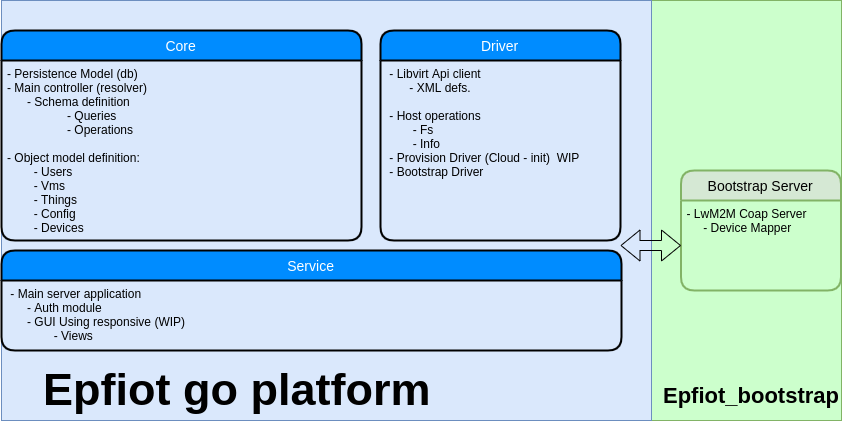
\includegraphics[width=5.5in]{figures/Application.png}
~\caption{Epfiot Overview}
\label{figure4.1}
\end{figure}
The following pages will show the implementation details taken for both parts.



\section{Epfiot platform}
\label{makereference4.2}

The main platform is a program written in Go that makes up most of the Epfiot Service.
It provides the following features:
\begin{itemize}
    \item Modern http API with basic authentication
    \item Sql as data model persistence
    \item Infrastructure management with near baremetal performance with USB passthrough for gpu computing
    \item Basic infra provisioning
    \item IoT oriented
    \item GUI
\end{itemize}

Being a program written from scratch made it necessary to do some architectural work in order to put all the logic together. The result was the creation of some modules differentiated by the function they perform within Epfiot.

\newpage
\subsection{Driver Module}
This module serves as an interface to different functionalities that Epfiot has to deal with, mostly related to host communication or the appliance itself. Some of them are:
\begin{itemize}
    \item \textbf{Virtual machine management}
    \item provisioning
    \item File system and OS operations
    \item Udp Client
\end{itemize}

\begin{figure}[h!]%t=top, b=bottom, h=here
\centering
    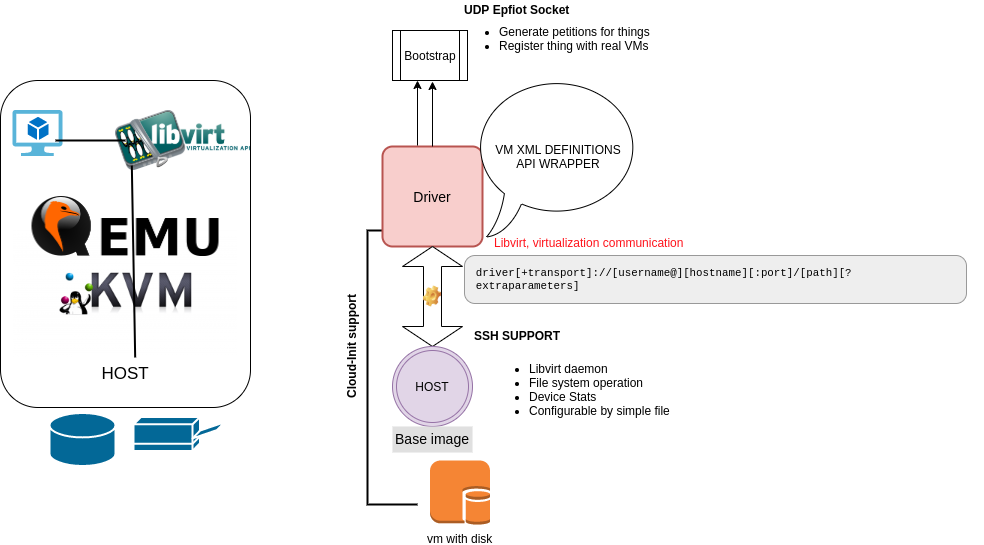
\includegraphics[width=6.0in]{figures/driver.png}
~\caption{Driver module overview}
\label{figure4.2}
\end{figure}

\textbf{Controller}

The protagonist of this module is the infrastructure Controller. This is the part of Epfiot that communicates with the host and handles the virtual machines. To perform this secure communication it uses SSH, which is compatible with Libvirt, the virtualization API with which Epfiot is able to control KVM AND QEMU from the host side.

It is important to know that the Controller is written in a decoupled form and activated by a configuration file, which means that it is possible to write another controller to put it to work with Epfiot!
This decision was made so that the project could evolve into newer forms of virtualization/containers in a near future without changing the rest of the functionality.
To build the Controller, a Golang interface is used in order to allow Epfiot to work with certain infrastructure functionalities that the driver has to implement.
The other Epfiot modules will work using this interface exposed by the controller.

\textbf{System operations} aka \textit{Utils}

With only the controller it is not possible to perform all the operations related to infrastructure. That is why the driver has a number of functions in the form of utilities to support the controller.

This part then takes care of some IO operation such as creating/copying/deleting disks or getting host information.

\textbf{Provisioning}

Epfiot is able to perform some basic provisioning operations. This part of the Driver module takes care or creating CD-ROMS with user settings (available via Epfiot API). This cdrom is inserted into the machine at its deployment and thanks to Cloud-Init it is able to perform actions such as creating users, installing packages, running scripts...

At the moment in Epfiot, the provisioning part only provides with the basic access credentials for the machine user and some basic networking however, is planned to expand the functionality in order to allow more operations.

\textbf{Udp communication}

Finally, the Driver module also handles Epfiot communications related to UDP. This is directly related to the bootstrapping part we'll see later.

The module acts as an UDP client to send certain information to the Epfiot Bootstrap process. This part of the module serves as an interface between Golang and C, something totally mandatory for use LWM2M implementations.

\newpage
\subsection{Service Module}

This section of Epfiot is responsible for serving an interface to the user.
Some of the purposes this module serves are as follows:
\begin{itemize}
    \item Authentication and security
    \item \textbf{ HTTP API endpoint}
    \item GUI
\end{itemize}

\begin{figure}[h!]%t=top, b=bottom, h=here
\centering
    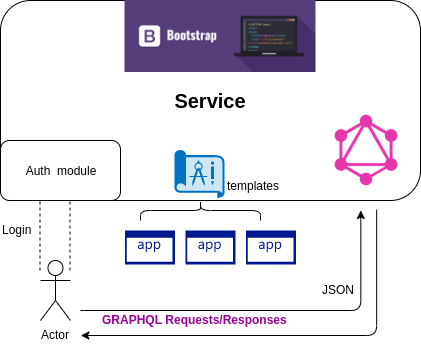
\includegraphics[width=4.0in]{figures/Service.png}
~\caption{Service module overview}
\label{figure4.3}
\end{figure}

\textbf{Epfiot API}

This module is responsible for exposing the operation api to the user.
Use Golang "net/http" native library to provide a fast we service. As you know, this module instead of using REST takes another perspective using a Graphql framework. This allows Epfiot to have a single endpoint where it is able to expose all operations through one schema. This scheme is described in Chapter \ref{makereference5.1}.

The user being aware of this scheme, is able to send json as a console to interact with Epfiot. This endpoint will respond with json objects depending on what the user asks.
\newpage

\textbf{Authentication}

Epfiot is a multitenant application, which means that it is capable of registering user and interacting with them. For this reason it is necessary to authenticate with Epfiot. 
The service module handles this authentication by maintaining a secure session for the user.

In the current version of Epfiot only a basic version of this module is implemented which allows you to identify the user and maintain their session.

\textbf{GUI}

To finish with this module we come to the part of the visual interface. The module has a visual system using the html/css/javascript templates offered by golang.

At the moment the most functional part of this visual interface is the console however, The logic that covers the rendering code is working and it is possible to make some graphic windows in a very simple way.



\newpage
\subsection{Core}

Core is the most fundamental part of Epfiot. The Epfiot Core can be understood as the heart of the application. In this module we find the code that controls the other modules (like the one for the Driver). In addition, the object model governing the entire application is defined here.

Some of the functions that this module performs are:
\begin{itemize}
    \item Objects definition (model)
    \item Database layer for model persistence
    \item Manage the data flow/operations of the entire application
\end{itemize}

\begin{figure}[h!]%t=top, b=bottom, h=here
\centering
    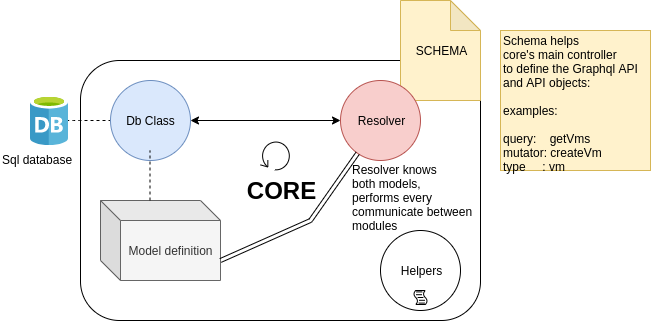
\includegraphics[width=5.5in]{figures/Core.png}
~\caption{Core overview}
\label{figure4.4}
\end{figure}

\textbf{Resolver}

Resolver is the class that handles the application. This code is in charge of receiving the actions dictated by the user through graphql, it is capable of of calling other modules to perform concrete actions. Inside this controller we can find many data definitions that the user is able to use in first instance (Chapter \ref{makereference5.1.1}).

As a design decision, Resolver save a pointer to the instance of the Driver module with which Epfiot is running.
As mentioned, Epfiot's architecture is decoupled and although at the moment there is only one driver for KVM, it is possible to implement any other as long as you keep the interface.


When the user makes an API call such as createVm, Epfiot uses the service module to handle any http session, right after that Resolve dictate what action to take.

\begin{figure}[h!]%t=top, b=bottom, h=here
\centering
    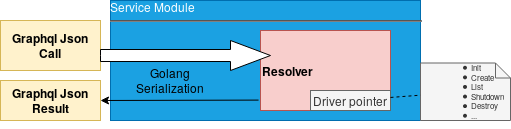
\includegraphics[width=5.0in]{figures/resolver.png}
~\caption{Service - Resolver - Driver Flow}
\label{figure4.5}
\end{figure}

\textbf{Data persistence}

As expected, one of the most important parts of the core is data persistence. Epfiot uses a relational model to store data and infrastructure status. To take this process, Core has a class that is exclusively in charge of communicate with the database.

When changes are made to the model, Resolver is able to access this storage layer in order to allow data persistence.

\textbf{Epfiot Model}

We refer to the model as the series of defined objects and the relationships they form with each other that Epfiot offers to the user in order to manage the infrastructure and IoT environment.

These objects that we can find inside Epfiot are the following:
\begin{itemize}
    \item \textbf{User}: The normal user entity that uses the application to know who own the environment.
    \item \textbf{Vm}: Representing the infrastructure, keeping information about the details of the machine and the status.
    \item \textbf{Devices}: Each of these objects represents the usb devices that has attached, storing information such as the bus number.
    \item \textbf{Things}: They represent the various IoT sensors you deploy and their relationship to the infrastructure.
    \item Config: The only purpose of this object is to save instance initialization options that could be reused.
\end{itemize}
\newpage

As you can see, the Epfiot model is quite simple and useful for the user to build his environment without any headache.


\begin{figure}[h!]%t=top, b=bottom, h=here
\centering
    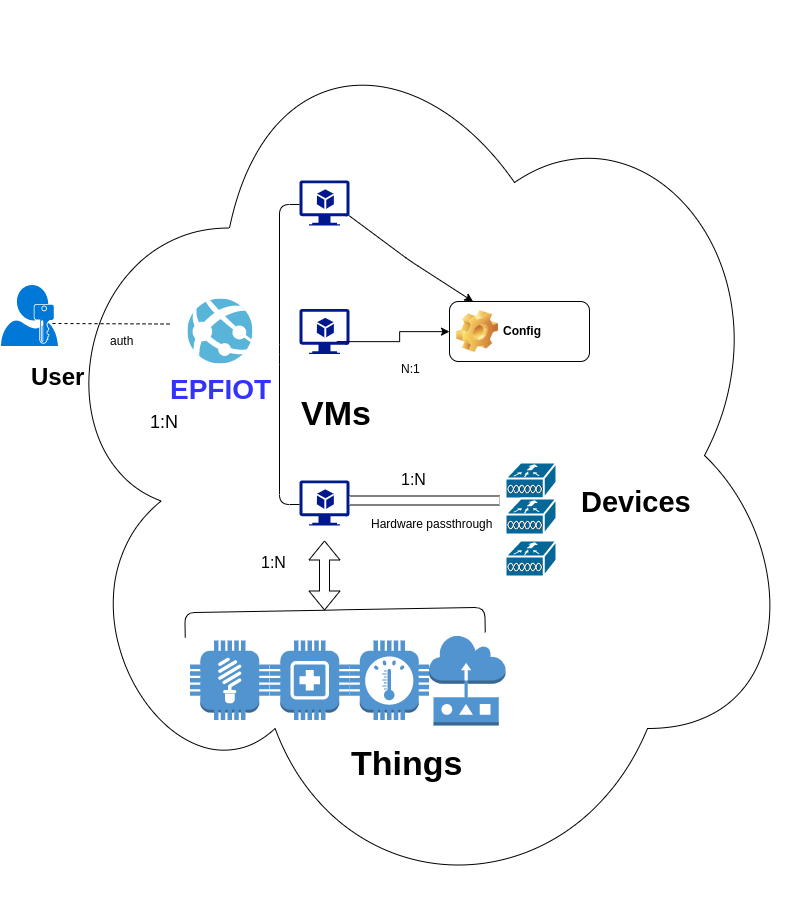
\includegraphics[width=6.0in]{figures/core_model.png}
~\caption{Epfiot Model Overview}
\label{figure4.6}
\end{figure}
\newpage


\section{Epfiot Bootstrap}
\label{makereference4.3}
In the Core part we have seen the underlying model of the application \ref{makereference4.2}. Specifically, there's part of this model called "things".
These objects not only serve to store information, but must actually be related to real sensors. To interact with those sensors it was decided the use of lwm2m2 protocol, an application layer for IoT device management.

Integrating Lwm2m2 into Epfiot was not an easy task, is a young protocol and there are still not many written implementations to use.
Finally Epfiot\_bootstrap was born a 'separate' project made for meet the requirements of lwm2m2 and take advantage of Eclipse Foundation's Wakaama implementation.

This part of Epfiot as its name suggest is based on the bootstrap service provided by lwm2m. A service with this implementation is launched in parallel to the main platform. A service with this implementation is launched in parallel to the main platform in charge of establishing relationships between the vms and the things.

\begin{figure}[h!]%t=top, b=bottom, h=here
\centering
    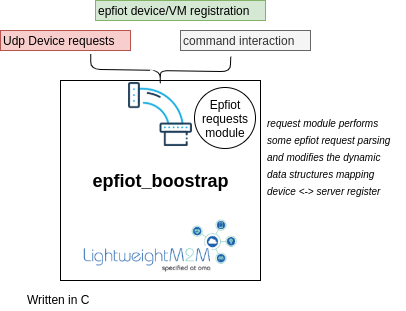
\includegraphics[width=5.0in]{figures/bootstrap.png}
~\caption{Epfiot\_bootstrap Overview}
\label{figure4.7}
\end{figure}

This process is listens to UDP packets and stores in memory the bootstrapping configuration for different sensors.
\newpage

Some of the actions performed by Epfiot bootstrap are the next:
\begin{itemize}
    \item Has implemented a protocol on udp built for Epfiot
    \item Store information about Epfiot vms and things
    \item When a sensor asks for bootstrapping configuration, Epfiot is able to configure it using its internal model
    \item Notify the main Platform that a client (sensor) has been registered and associated with certain vm
\end{itemize}

\begin{figure}[h!]%t=top, b=bottom, h=here
\centering
    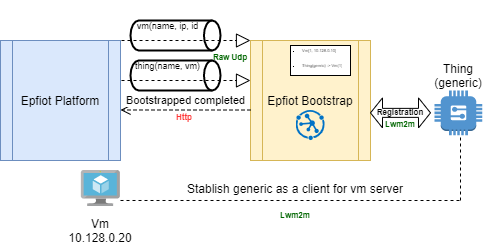
\includegraphics[width=6.5in]{figures/Epfiot_bootstrap_example.png}
~\caption{Epfiot\_bootstrap example}
\label{figure4.8}
\end{figure}


% +--------------------------------------------------------------------+
% | Sample Chapter 3
% +--------------------------------------------------------------------+

\cleardoublepage

% +--------------------------------------------------------------------+
% | Replace "This is Chapter 3" below with the title of your chapter.
% | LaTeX will automatically number the chapters.
% +--------------------------------------------------------------------+

\chapter{Interfaz Usuario}
\label{makereference5}

Here are more examples of referring to previous sections.  In
Chapter~\ref{makereference} there were several sections, including
section~\ref{makereference1.1}, section~\ref{makereference1.2},
and section~\ref{makereference1.3}.

Likewise, in Chapter~\ref{makereference2}, there are
sections~\ref{makereference2.1} and ~\ref{makereference2.2}.




% +--------------------------------------------------------------------+
% | Replace \section headings below with the title of your
% | subsections.  LaTeX will automatically number the subsections 1.1,
% | 1.2, 1.3, etc.
% +--------------------------------------------------------------------+

\section{Types}
\label{makereference5.1}

In this paragraph, we want to refer to Fig.~\ref{figure1}
mentioned at the beginning of this chapter.  We also refer to the
Table~\ref{table1}.

\section{Queries}
\label{makereference5.2}

In this section, we refer back to text mentioned in
Section~\ref{makereference1.1} on page~\pageref{makereference1.1}.

\section{Mutations}
\label{makereference5.3}

Here's an example of a citation to a single
work.~\citet{CT:Weiner:1999} It's also possible to make multiple
citations.~\citet{CT:Phillips:1985, ARP:Loy:1974}

% +--------------------------------------------------------------------+
% | Sample Chapter 3
% +--------------------------------------------------------------------+

\cleardoublepage

% +--------------------------------------------------------------------+
% | Replace "This is Chapter 3" below with the title of your chapter.
% | LaTeX will automatically number the chapters.
% +--------------------------------------------------------------------+

\chapter{Examples}
\label{makereference6}

In this section we're going to explain a few use cases that could be actually applied using Epfiot application.

With these examples, a greater understanding is sought for the reader of how Epfiot works. It is also intended to serve as a guide for beginners in the use of the application.


The examples in order are as follows:
\begin{itemize}
    \item \textbf{Scenario}: Before moving on to the examples, the used technical scenario will be described.
    \item \textbf{Authentication and basic use}: This example will explain the basics of Epfiot. A user of the application logs in and creates a virtual machine.
    \item \textbf{Using vms and accelerators}: A more advanced user decides to use Epfiot and its usb accelerators. He creates two virtual machines and decides to attach an accelerator to one with the purpose of compare the performance.
    \item \textbf{Taking care of things}: This user wants to mount a complete stack using Epfiot: It will create virtual machines, assign accelerators, create things and see how the model works.
\end{itemize}

\newpage
\section{Scenario}
\label{makereference6.1}

We're going to use a simple scenario to deal with the examples in Epfiot.
Our main network will be a wireless wifi network, managed by a normal access point/router with dhcp over 192.168.1.0/24. We are going to install our NUC5i5RYK in this network, to avoid problems we are going to put a static ip 192.168.1.141.

In our NUC it is necessary to have a Linux installed an the KVM hypervisor, In Chapter \ref{makereference3.1} are detailed the necessary packages for an Epfiot ecosystem from the host point of view. 
A series of installation scripts are available in Epfiot main repository \cite{epfiot_install} to execute the following steps:

\begin{itemize}
    \item Create the private network for Epfiot (in our case using libvirt routed feature), in this case 10.128.0.0/24.
    \item Create a virtual machine with The Epfiot Appliance with a static ip (10.128.0.141).
    \item Start the service.
\end{itemize}

Finally the scenario looks like this        :

\begin{figure}[h!]%t=top, b=bottom, h=here
\centering
    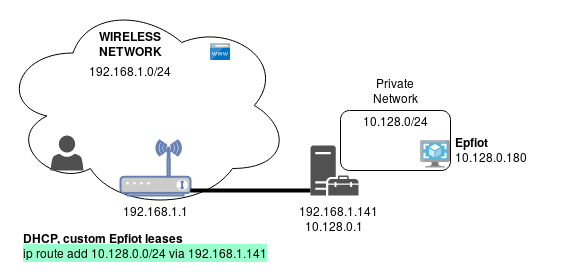
\includegraphics[width=5.5in]{figures/Epfiot_example.png}
~\caption{Epfiot Scenario}
\label{figure6.1}
\end{figure}

\newpage
\section{Authentication and basic use}
\label{makereference6.2}

Epfiot is user based, at the moment there is no public service dedicated to Epfiot and the installation is private.
For the alpha version (current) there are a number of example users already created to be able to test the application. 

The user Charlie@gmail.com has access to the Epfiot alpha and proceeds to enter into the application. Epfiot has an authentication system so you have to enter a username and password if you want to interact.
\begin{figure}[h!]%t=top, b=bottom, h=here
\centering
    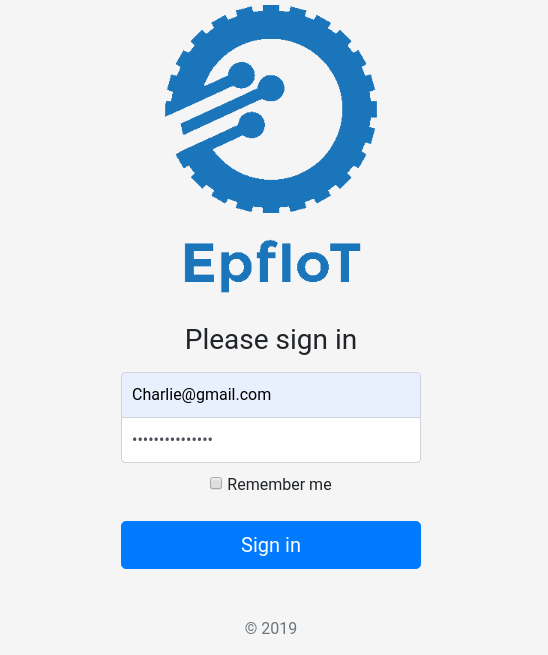
\includegraphics[width=3.5in]{figures/login.png}
~\caption{Epfiot Login}
\label{figure6.2}
\end{figure}

Once inside the application, the alpha version of epfiot provides you with a graphql console.
Charlie can write in this console the operations already seen in Chapter \ref{makereference5}.

This example is a basic use of Epfiot, the user just wants to create a machine in an edge environment.

\newpage
Therefore he will use the createvm operation adding a configuration to be able to enter the machine:

\begin{figure}[h!]%t=top, b=bottom, h=here
\centering
    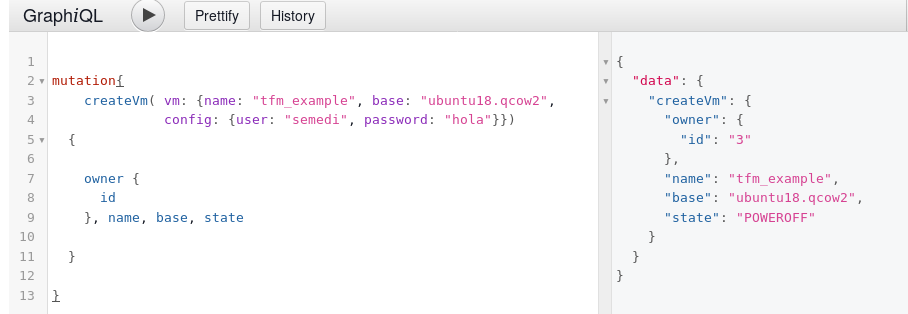
\includegraphics[width=6.5in]{figures/create_vm.png}
~\caption{Vm creation}
\label{figure6.3}
\end{figure}

As you can see, the user is asking for specific return values, such as the status of the machine, its name or even the owner's ID.
When the machine has been created, the user is ready to perform some basic operations like for example turn on the vm:


\noindent\fbox{%
    \parbox{\textwidth}{%
        mutation {
            powerOn(vmID:1){}
        }
    }%
}

Although the command itself gives you a clear feedback on whether the operation has been completed successfully or not, the user probably wants to know more information about his machine. Charlie uses the getvms command to see what is the current status:

\begin{figure}[h!]%t=top, b=bottom, h=here
\centering
    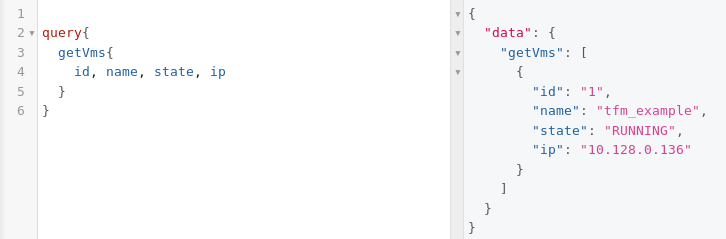
\includegraphics[width=5.5in]{figures/get_vms.png}
~\caption{Vm creation}
\label{figure6.4}
\end{figure}

At this point, Charlie is able to use his new machine in the edge environment.  It is important to note that the machine is accessible through ssh, using as credentials those which are already provided in the creation of the machine. In this example, the user will build everything on his own and only uses Epfiot to create basic infrastructure.

\newpage
\section{Using vms and accelerators}
\label{makereference6.3}

In this example Charlie is going to use one of the most important features of Epfiot as it is to be able to use real hardware accelerators with your machine.

To do this, he's going to use two machines.


\begin{itemize}
    \item The first is the one used in the first example. For this machine (10.128.0.136) Charlie will attach the Google Coral accelerator to test if there is any performance improvement when making inference.
    \item He will create another machine (just like the first example), this time without any device attached. The purpose is to see if there was really a deterioration in the speed compared to the previous test.
\end{itemize}

First of all, Charlie should check with usb devices are available on the host, for this Epfiot has the getusb operation, which gives you a list of the physical devices:
\begin{figure}[h!]%t=top, b=bottom, h=here
\centering
    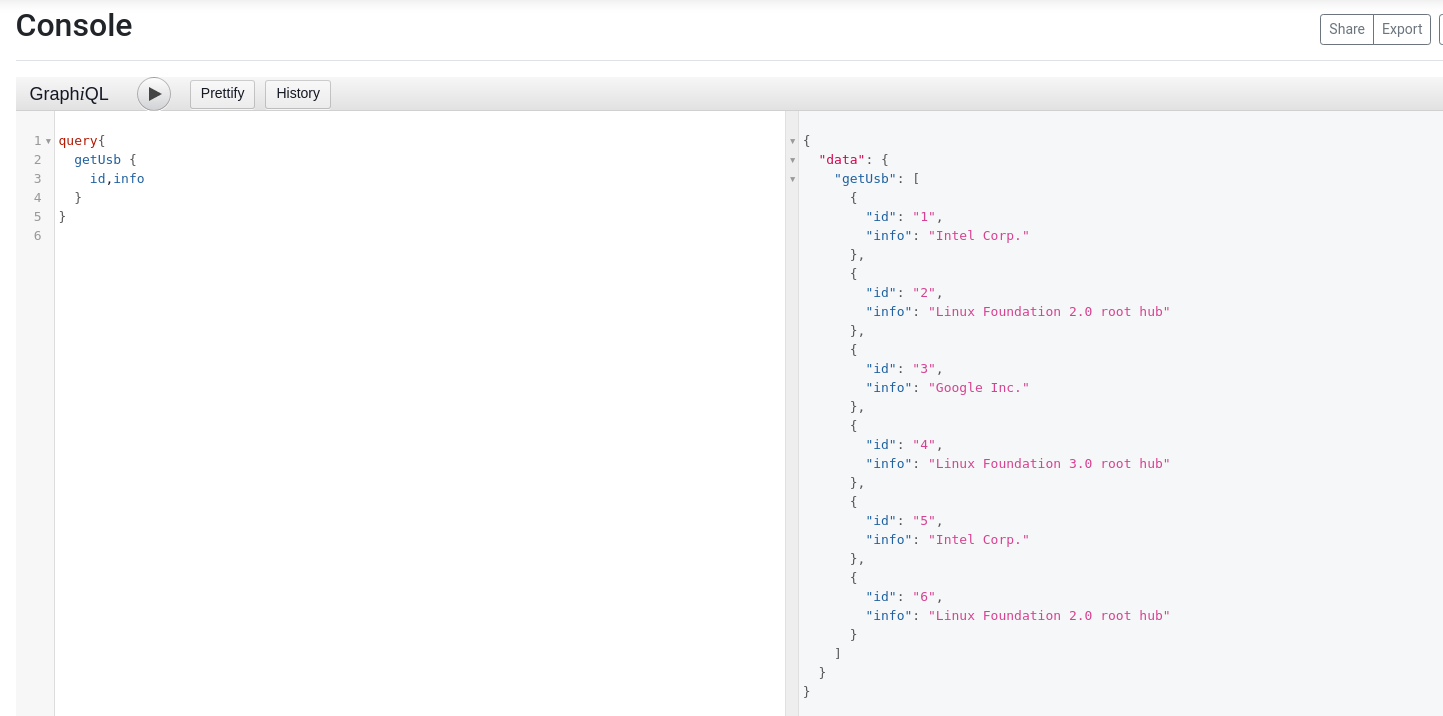
\includegraphics[width=7.0in]{figures/lsusb.png}
~\caption{lsusb operation}
\label{figure6.5}
\end{figure}
\newpage

In this case, we know that Google is the manufacturer of the device, therefore our usb accelerator has de ID 3 as seen in the picture \ref{figure6.5}.

Once we know the device ID, we need to find the ID associated to our machine as well. To do this we can use the \textbf{getVms} operation already done in the figure \ref{figure6.4} where we showed some interesting information of the machine such as the id, status or the ip itself.

If we look at the \textbf{attachDevice} header in Chapter \ref{makereference5.3}, you can see that it needs two arguments which are the IDs already obtained:
\begin{figure}[h!]%t=top, b=bottom, h=here
\centering
    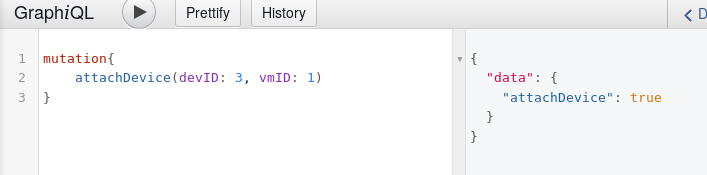
\includegraphics[width=4.5in]{figures/attach_dev.png}
~\caption{attachdevice operation}
\label{figure6.6}
\end{figure}

Epfiot quickly reports that the operation has been successfully completed by returning a boolean value, however Charlie wants to check it himself.
The following image shows the command that Charlie executed on his cmd in order to check that the machine is actually running, it has the user and password indicated by Epfiot and it has a usb accelerator attached:

\begin{figure}[h!]%t=top, b=bottom, h=here
\centering
    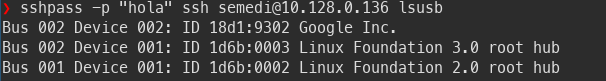
\includegraphics[width=4.5in]{figures/attach_device_ls.png}
~\caption{Charlie checking the machine}
\label{figure6.7}
\end{figure}

As you can see, the machine is operational and has the Google coral installed!

Now that the first machine is ready, Charlie proceeds to create another machine just like the first one, this time without attaching any additional device.
The result is a machine using the Google coral accelerator and another one that will use virtual cpu.
\newpage

\textbf{Using Google Coral Accelerator}

Charlie decides to test if he can really use Google's accelerator from a virtual machine.
To do this, he runs the example code of Google Coral on the machine that has the device attached and gets the following results:

\begin{figure}[h!]%t=top, b=bottom, h=here
\centering
    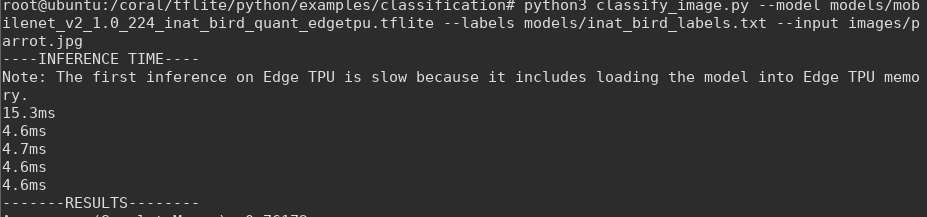
\includegraphics[width=6.5in]{figures/vm_dev_inference.png}
~\caption{Test vm using Google Coral}
\label{figure6.8}
\end{figure}

Charlie gets pretty good results ~4.6ms.

\textbf{Using Virtual Cpu}

Now Charlie is preparing to do the same test using the other machine without the aid of any additional device:

\begin{figure}[h!]%t=top, b=bottom, h=here
\centering
    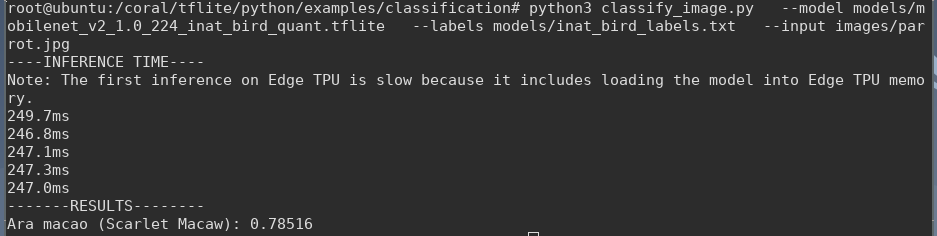
\includegraphics[width=6.5in]{figures/vm_nodev_inference.png}
~\caption{Test vanilla vm}
\label{figure6.9}
\end{figure}

It's easy to see the difference in the results, Charlie gets a speed of ~247ms worsening drastically the results obtained in the previous test.

With this test Charlie has learned that Epfiot's feature of attaching real devices is very useful in certain occasions such as those that could happen in an edge environment.
\newpage
\section{Taking care of things}
\label{makereference6.4}

Once Charlie knows about the real device management feature, he decides to deploy some sensors with which he will build his Internet of Things stack using the infrastructure already created.

For the above test he created two machines, quickly he realizes that he would only need one machine for his stack so he deletes the first one:

\begin{figure}[h!]%t=top, b=bottom, h=here
\centering
    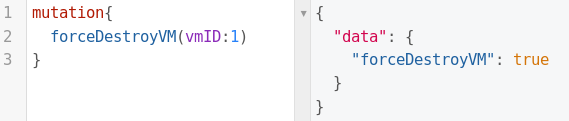
\includegraphics[width=4.5in]{figures/force_destroy.png}
~\caption{destroy a machine}
\label{figure6.10}
\end{figure}

Force destroy operation \ref{makereference5.3} allows you to abruptly remove a machine.

Counting only with one machine, he realizes that he does not remember the given name to the machine. 
For his new test he wants to know the name of the machine, its ip, memory and virtual cpu.

Thanks to graphql, Epfiot allows you to use queries asking only for the desired values:

\begin{figure}[h!]%t=top, b=bottom, h=here
\centering
    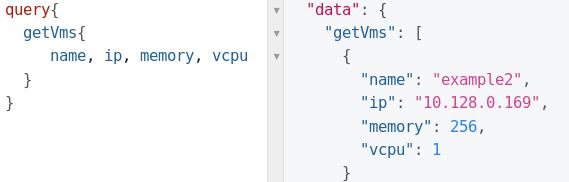
\includegraphics[width=5.5in]{figures/concrete_getvm.png}
~\caption{specific getvm operation}
\label{figure6.11}
\end{figure}

\newpage
Looking at Epfiot's log, he sees that something has happened to the machine. To handle the sensors, Epfiot register the infrastructure on its bootstrapping server. Therefore his "example2" machine is ready to be used with new sensors:

\begin{figure}[h!]%t=top, b=bottom, h=here
\centering
    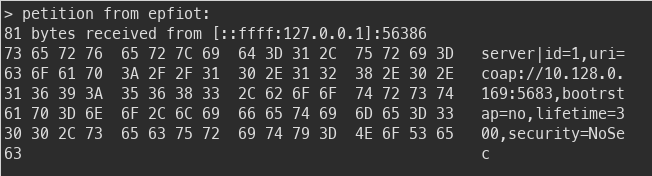
\includegraphics[width=6.5in]{figures/bs_server_log.png}
~\caption{bootstrap server log}
\label{figure6.12}
\end{figure}

This Epfiot functionality allows you to register sensors directly with your infrastructure. Epfiot saves the device information in its bootstrap server, so that as soon as the device enters into the network it can be configured with the setting of the newly created server automatically.
To do this, Charlie creates a new test device on epfiot:

\begin{figure}[h!]%t=top, b=bottom, h=here
\centering
    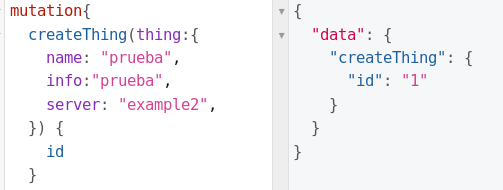
\includegraphics[width=5.5in]{figures/create_thing.png}
~\caption{Create a thing}
\label{figure6.13}
\end{figure}

The "prueba" sensor is now linked to the example2 machine! At least from the point of view of the Epfiot mode (See Figure \ref{figure6.14}).For the device to be automatically configure it must first be deployed on the network where Epfiot is located.

Following the figure \ref{figure6.1}, Charlie deploys his new sensor in the wireless network (192.168.1.0/24). Remember that since the router have a table for 10.128.0.0/24 network, it is possible to access the Epfiot private network and reach the allocated vms.
\newpage

\begin{figure}[h!]%t=top, b=bottom, h=here
\centering
    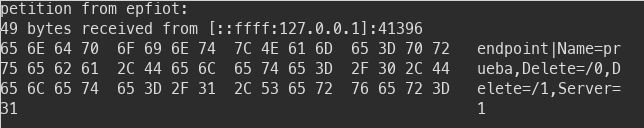
\includegraphics[width=5.5in]{figures/bs_endpoint_log.png}
~\caption{Epfiot bootstrap device registration}
\label{figure6.14}
\end{figure}

With Epfiot ready, Charlie turns on his new lwm2m sensor into the network and watches the generated log:

\begin{figure}[h!]%t=top, b=bottom, h=here
\centering
    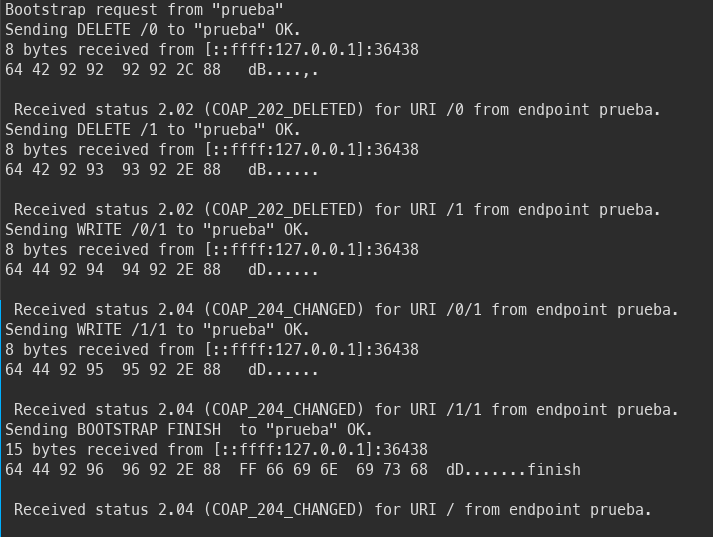
\includegraphics[width=5.5in]{figures/bs_endpoint_log2.png}
~\caption{Epfiot psychical sensor detected}
\label{figure6.15}
\end{figure}

Epfiot discovers this new sensor "prueba" and proceeds to send its new bootstrapping configuration.
In the alpha phase Epfiot follows these steps:
\begin{itemize}
    \item Delete /0 object
    \item Delete /1 object
    \item write the 'master' server configuration (In this case 10.128.0.169).
\end{itemize}
\newpage

To finish his test, Charlie checks if anything has happened on the deployed server, he gets the following results

\begin{figure}[h!]%t=top, b=bottom, h=here
\centering
    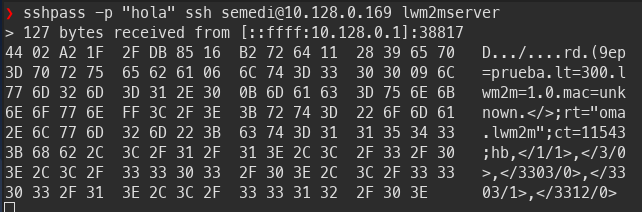
\includegraphics[width=6.5in]{figures/bs_endpoint_log3.png}
~\caption{Deployed vm receiving information about a new device}
\label{figure6.16}
\end{figure}

The "prueba" device is now attached to the virtual machine previously created! All made simple with Epfiot, now from his machine, Charlie can continue to interact remotely with his new sensor.

Since Epfiot has configured the "prueba" sensor, Charlie can also see which devices are active (they are in the network and have been bootstrapped by the application):


\begin{figure}[h!]%t=top, b=bottom, h=here
\centering
    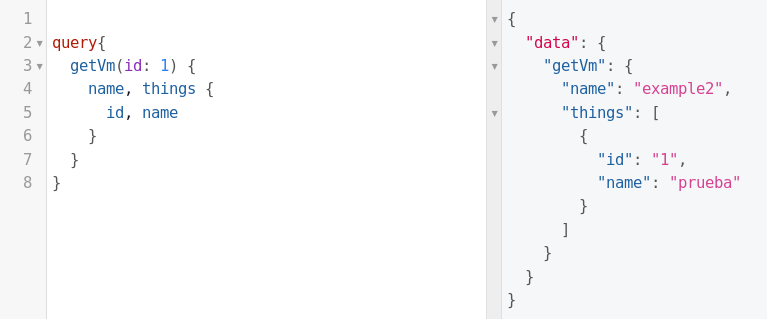
\includegraphics[width=6.5in]{figures/attached_thing.png}
~\caption{The bootstrapped thing}
\label{figure6.17}
\end{figure}

% +--------------------------------------------------------------------+
% | Sample Chapter 7
% +--------------------------------------------------------------------+

\cleardoublepage

% +--------------------------------------------------------------------+
% | Replace "This is Chapter 2" below with the title of your chapter.
% | LaTeX will automatically number the chapters.
% +--------------------------------------------------------------------+

\chapter{Conclusions and Future work}
\label{makereference7}
\section{Conclusions}
\label{makereference7.1}

This work aimed to study the feasibility of having dynamic infrastructure in a cloud model adapted to today's needs, in a environment of very limited resources such as the Internet of Things and Edge computing.

It was therefore decided to implement and design a lightweight, energy-saving appliance. The result is Epfiot and the following functionalities were achieved:
\begin{itemize}
    \item Web multi tenant application, following the basics cloud principles with a data storage model and a visual interface.
    \item Infrastructure management with near baremetal performance and provisioning system.
    \item Ability to use real use accelerators, attaching them dynamically to the infrastructure.
    \item System oriented to the IoT Paradigm, using new protocols such as Lwm2m to have an easy handling of the sensors withing the environment.
\end{itemize}

With these features in mind, it can be said that the objectives have been satisfactorily achieved. It is possible to use such a platform in an Edge environment.

Finally, it should be noted that a hypervisor like kvm is undoubtedly effective for this kind of project, but emulators such as Qemu should be replaced in order to achieve lower overhead and lighter guests. However, it is safe to say that by using this type of technology a quite useful virtual environment can be guaranteed for the end user.

\newpage
\section{Future Work}
\label{makereference7.2}

Developing a product like Epfiot has been a very hard work due to the complexity involved. To be able to build this type of platform you have to take many factors into account, as the application is very large and many concepts such as security have to be properly considered.

With this in mind, Epfiot achieved the basic objectives for which the project was designed, however some tasks can be contemplated in order to improve the project:

\begin{itemize}
    \item \textbf{Stability \& maintenance}: Like any application this one also requires maintenance and bug hunting.
    \item \textbf{Improve security}: For the development of the project, some protocols have been made and the should have better security using encryption.
    \item \textbf{Better infra provisioning}: Epfiot allows you to make a basic provision for the machines, it would be useful to improve this part
    \item \textbf{Configurable thing bootstrap}: Epfiot performs a series of static steps to configure the devices, thanks to Lwm2m this part can be easily customized by the user in the future.
    \item \textbf{Expand the graphic interface}: As the moment there is only the basic part as is was not withing the scope of the project.
\end{itemize}

It is important to mention that Epfiot leaves open the possibility of developing more than one virtualization driver for the application. This means that it is possible to expand the project with some new technology quite simply. Therefore a good option in the future could be to implement another driver and compare performance with the current one.
%% +--------------------------------------------------------------------+
% | Sample Chapter
% |
% | This file provides examples of how to
% | - insert a figure with a caption
% | - construct a table with a caption
% | - create subsections within the chapter
% | - insert a reference to a Figure or Table
% | - make a citation
% +--------------------------------------------------------------------+

\cleardoublepage

% +--------------------------------------------------------------------+
% | Replace "Chapter Title" below with the title of your chapter.  LaTeX
% | will automatically number the chapters.
% +--------------------------------------------------------------------+

\chapter{Introduction}
%\label{ch:Introducción}
\label{makereference}

In this chapter, there will be examples of various features you
may want to incorporate into your document. Here's an example of a
figure inserted into the text:

\begin{figure}[htb]%t=top, b=bottom, h=here

    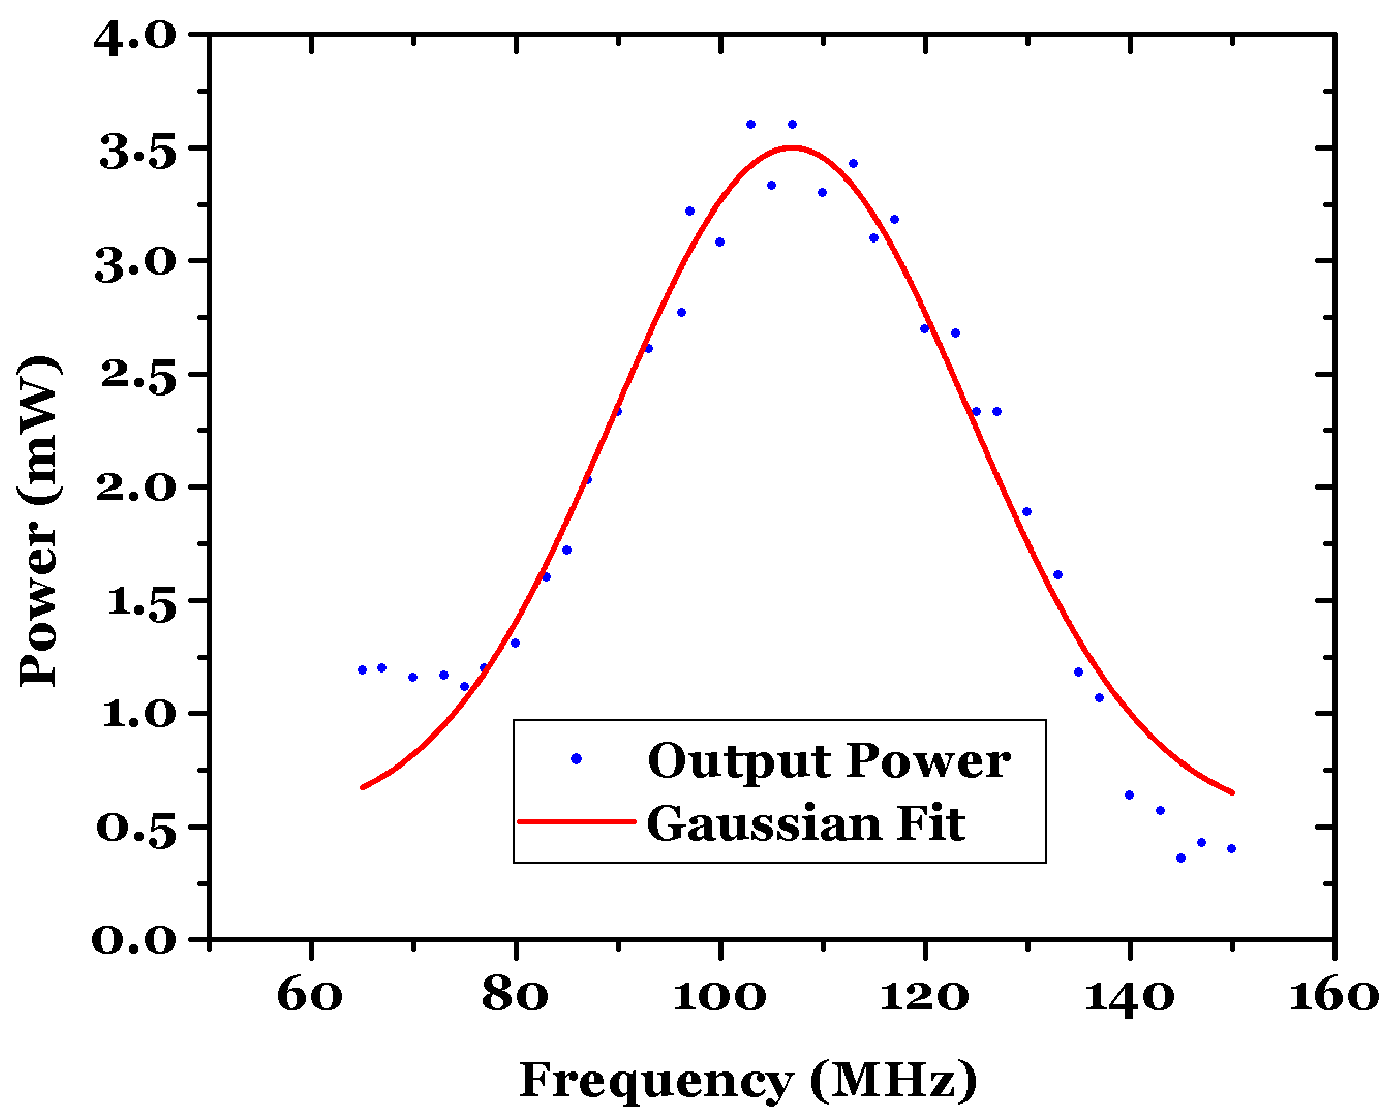
\includegraphics[height=2.5in]{figures/graph.png}

    \caption[Optional: Short caption to appear in List of
    Figures]{Full caption to appear below the Figure}

    \label{figure1}
\end{figure}

% +--------------------------------------------------------------------+
% |To create cross-references to figures, tables and segments
% |of text, LaTeX provides the following commands:
% |   \label{marker}
% |   \ref{marker}
% |   \pageref{marker}
% | where {marker} is a unique identifier.
% |
% | In the line above, we use \label{figure1} to mark a location
% | we wish to refer to later.  LATEX replaces \ref by the number of
% | the chapter, section, subsection, figure, or table after which the
% | corresponding \label command was issued. \pageref prints the page
% | number of the page where the \label command occurred.
% |
% +--------------------------------------------------------------------+

Here is an example of a Table:

\begin{table}

% +--------------------------------------------------------------------+
% | We include the command \begin{center} to center the table
% | horizontally on the page.  Note use of the command \end{center}
% | to turn off centering after the table is defined.
% +--------------------------------------------------------------------+
    \begin{center}

% +--------------------------------------------------------------------+
% | The table is created with this command
% |
% | \begin{tabular}[pos]{table spec}
% |
% | The "pos" argument specifies the vertical position of the table relative to
% | the baseline of the surrounding text.  Use t, b, or c to specify alignment
% | at the top, bottom, or center.
% |
% | The "table spec" command defines the format of the table
% |   l for a column of left-aligned text
% |   r for a column of right-aligned text
% |   c for centered text
% |   p{width} for a column containing justified text with line breaks
% |   | for a vertical line
% +--------------------------------------------------------------------+

    \begin{tabular}[c]{|c|c|c|}
        \hline
        Column 1 Heading & Column 2 Heading & Column 3 Heading \\
        \hline
        Col 1 Row 1 & Col 2 Row 1 & Col 3 Row 1\\
        Col 1 Row 2 & Col 2 Row 2 & Col 3 Row 2\\
        Col 1 Row 3 & Col 2 Row 3 & Col 3 Row 3\\
        \hline
    \end{tabular}
    \caption{Caption to appear below the table}
    \label{table1}
   \end{center}
\end{table}

% +--------------------------------------------------------------------+
% | Replace \section headings below with the title of your
% | subsections.  LaTeX will automatically number the subsections 1.1,
% | 1.2, 1.3, etc.
% +--------------------------------------------------------------------+

\section{Motivation}
\label{makereference1.1}

In this paragraph, we want to refer to Fig.~\ref{figure1}
mentioned at the beginning of this chapter.  We also refer to the
Table~\ref{table1}.

\section{Purposes}
\label{makereference1.2}

In this section, we refer back to text mentioned in
Section~\ref{makereference1.1} on page~\pageref{makereference1.1}.

\section{Structure of the project}
\label{makereference1.3}

Here's an example of a citation to a single
work.~\citet{CT:Weiner:1999} It's also possible to make multiple
citations.~\citet{CT:Phillips:1985, ARP:Loy:1974}

%% +--------------------------------------------------------------------+
% | Sample Chapter 7
% +--------------------------------------------------------------------+

\cleardoublepage

% +--------------------------------------------------------------------+
% | Replace "This is Chapter 2" below with the title of your chapter.
% | LaTeX will automatically number the chapters.
% +--------------------------------------------------------------------+

\chapter{Conclusions and future work}
\label{makereference9}

In this chapter, I want to refer to Chapter~\ref{makereference},
so I'm going to use the slash ref command along with the
"makereference" label which I assigned back at the beginning of
Chapter 1.


% +-------------------------------------------------------------------------+
% | References                                                              |
% +-------------------------------------------------------------------------+

% +-------------------------------------------------------------------------+
% | In order for WinEDT to index references correctly, it has to know where |
% | the file resides.  The following command is prefaced by %, and will be  |
% | ignored completely by LaTeX.  However, WinEDT will use this line to     |
% | access the external .bib bibliography file.  Also note that WinEDT can  |
% | read file path names with either "\" or "/" - LaTeX, however, doesn't   |
% | like "\", so it's easier to store a path name in the "Unix" style.      |
% +-------------------------------------------------------------------------+

%Included for Gather Purpose only.  Do NOT uncomment:
%input "references.bib"

% +--------------------------------------------------------------------+
% | This template uses the BibTeX program to format references.  The
% | 3 lines below create a separate Bibliography section and add
% | an entry for "Bibliography" to the Table of Contents.  The actual
% | data for your references (author, title, journal, date, etc.) are
% | entered in the references.bib file.  See that file for information
% | on how to enter references.
% +--------------------------------------------------------------------+

\bibdata{references}
\bibliography{references}
\addcontentsline{toc}{chapter}{Bibliography}

% +--------------------------------------------------------------------+
% | Finally, we generate the appendix.  To add or delete appendices,
% | add or remove the line
% |
% |     \input{appendixX.tex}
% |
% | where "X" is the letter designation of the Appendix (A, B, C, etc.)
% | You should have one \input{appendixX.tex} line and a corresponding
% | file appendixX.tex for each appendix.                                 |
% +--------------------------------------------------------------------+

\appendix
% +--------------------------------------------------------------------+
% | Appendix A Page (Optional)                                         |
% +--------------------------------------------------------------------+

\cleardoublepage

\chapter{Title for This Appendix}
\label{Appendix:Key1}


% +--------------------------------------------------------------------+
% | Enter text for your Appendix page in the space below this box.     |
% |                                                                    |
% +--------------------------------------------------------------------+

% +--------------------------------------------------------------------+
% | Appendix B Page (Optional)                                         |
% +--------------------------------------------------------------------+

\cleardoublepage

\chapter{Title for This Appendix}
\label{Appendix:Key2}

% +--------------------------------------------------------------------+
% | Enter text for your Appendix page in the space below this box.     |
% |                                                                    |
% +--------------------------------------------------------------------+


\end{document}
